
Now, in the preamble of your code, input {\em myFigures.tex} in the
same manner as you input {\em titlepage.tex}.  Now we are ready to add
the main body of the thesis.  Initiate the main body of your document
by calling the {\bf$\backslash$mainmatter} command.  Next, call the
figures that you have defined and compile.  Note, once you add a
chapter, you can remove {\bf$\backslash$thispagestyle\{plain\}} which
precedes the {\bf$\backslash$mainmatter} command.

\vspace{-0.3in}
{\singlespace
\begin{verbatim}
\documentclass[12pt,letterpaper,oneside]{book}
\usepackage{afitThesis}
\graphicspath{{..\Figures}}
\input{Preamble/titlepage}
%% myFigures.tex
% A common file to store all figure definitions
%
% In preparing your thesis, one of the first things you should do is
% organize your figures.  Then, one of the last things you'll do is
% reorder your figures so they display where you want them to in the
% text.  Organizing figure definitions in a common files helps:
%
%   1. Write new figures using earlier examples.
%
%   2.  Isolate code and minimize the risk of introducing bugs in the
%   final editing process.  Trust me, moving around just one line of
%   code is easier.
%
%   3.  Reuse figures in other papers.  <=== the best reason!
%
% Note command names can not include numbers and special characters.
%
% To make the file more searchable, use naming conventions that map
% the graphics filename labSetup.jpg to the command name \figlabSetup to the
% figure label fig:labSetup.
% 

\newcommand{\figMyFirstLaTeX}{\begin{figure}[tbp]
 \begin{center}
    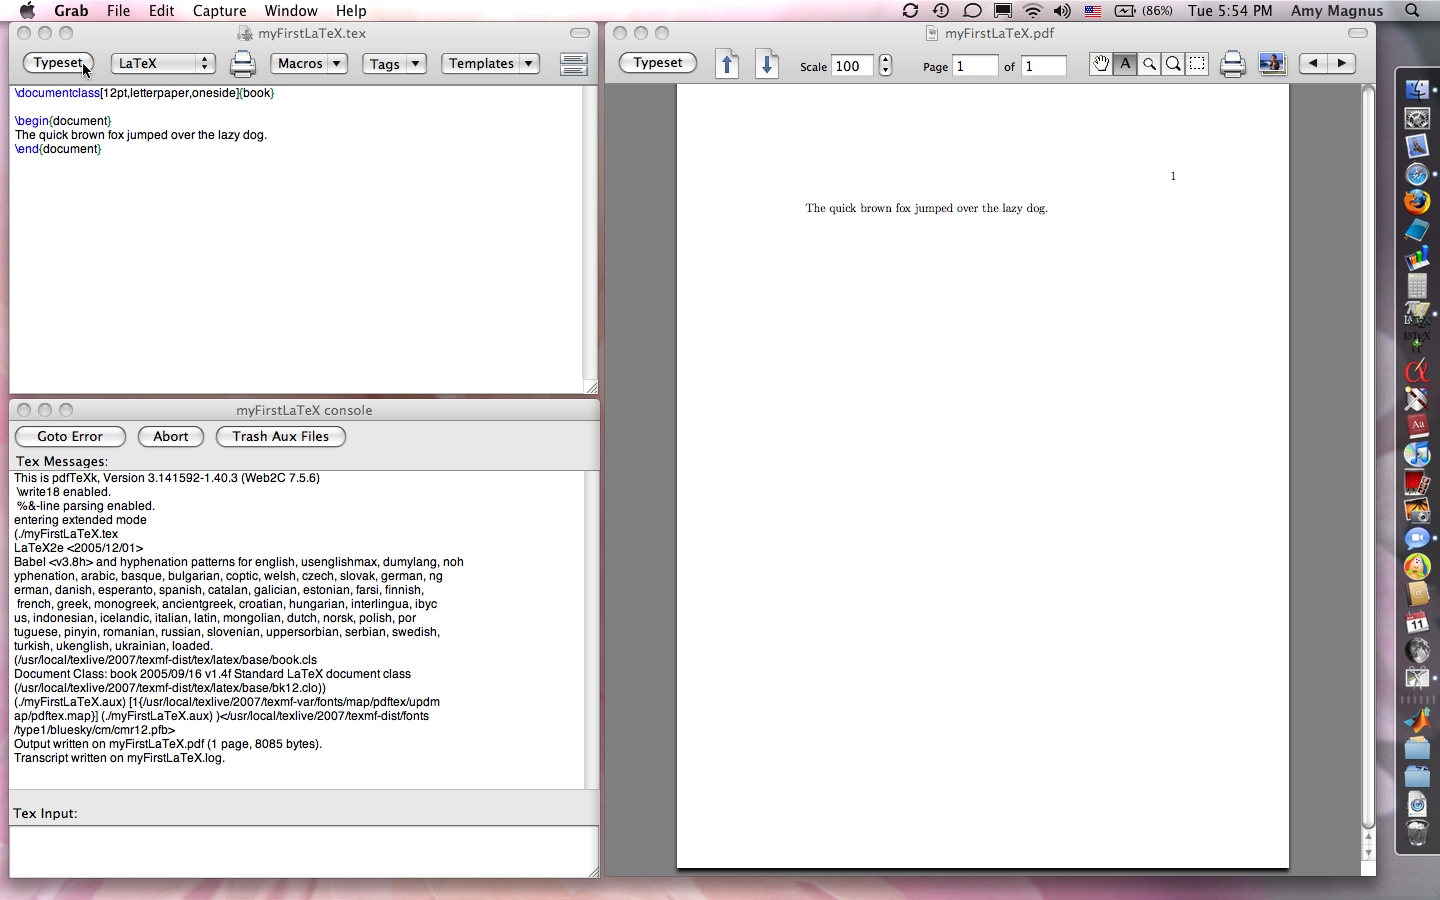
\includegraphics[width=6in]{myFirstLaTeXCursor}
     \caption[\LaTeX\ a very simple document]{Compile a very simple document.}
     \label{fig:MyFirstLaTeX}
 \end{center}
 \vspace{-0.2 in}
\end{figure}
}


\newcommand{\figafitStyle}{\begin{figure}[tbp]
 \begin{center}
    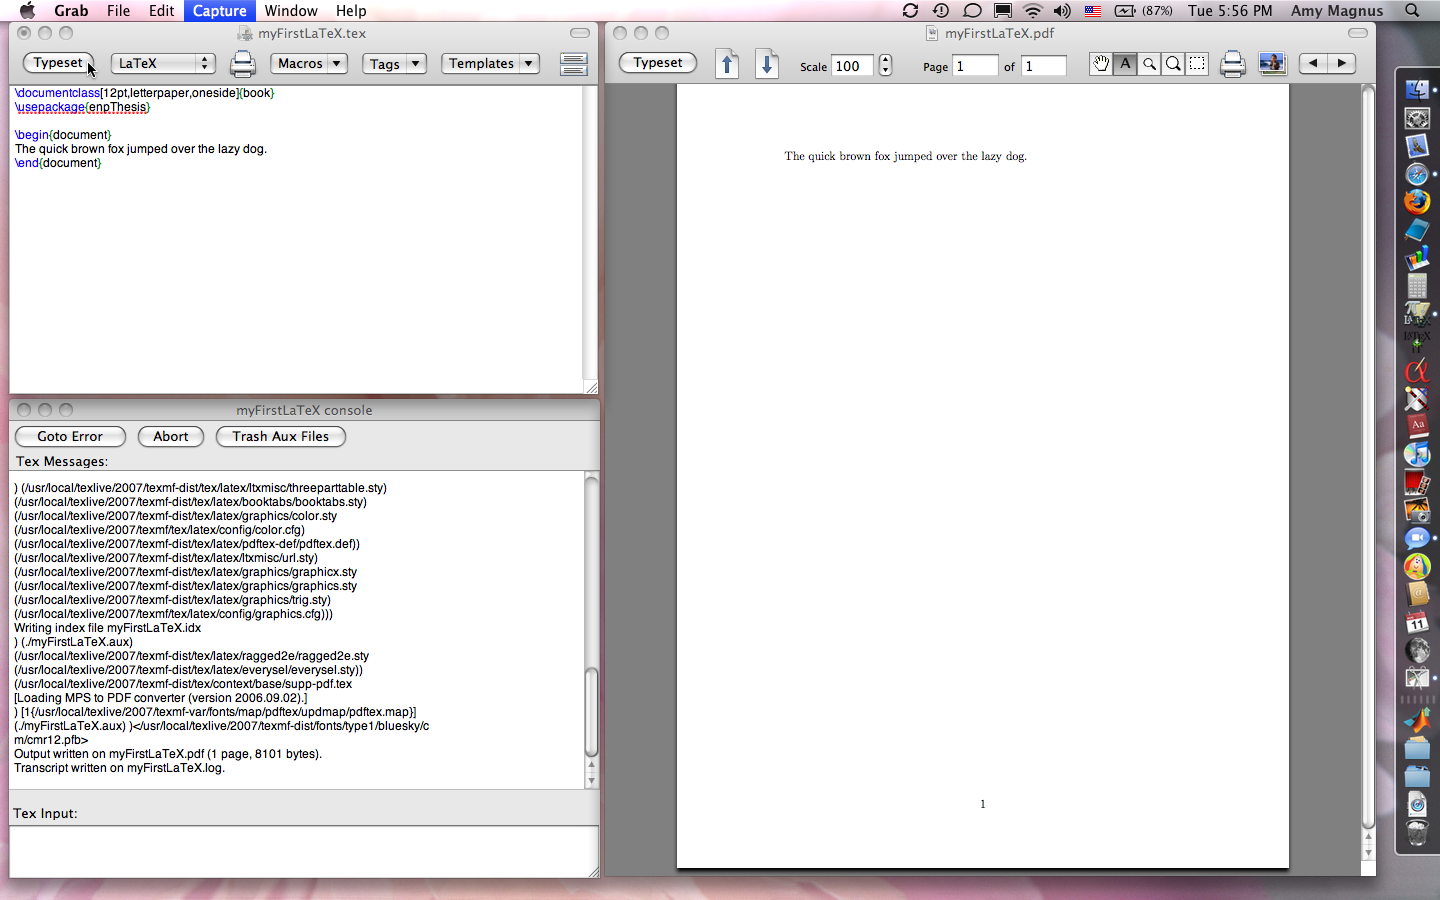
\includegraphics[width=6in]{myFirstLaTeXafit}
     \caption{Recompile using afitThesis.sty, the AFIT
     thesis style file.}
     \label{fig:afitStyle}
 \end{center}
\end{figure}
}


\newcommand{\figtitlePage}{\begin{figure}[tbp]
 \begin{center}
    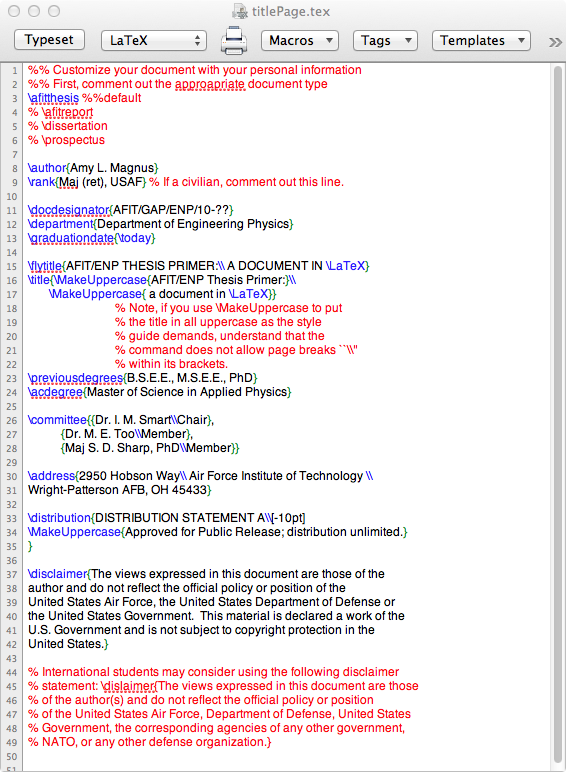
\includegraphics[width=6in]{titlePage}
     \caption{Enter student data in titlePage.tex to customize the
     document's first pages.}
     \label{fig:titlePage}
 \end{center}
\end{figure}
}

\newcommand{\figmyFlypage}{\begin{figure}[tbp]
 \begin{center}
    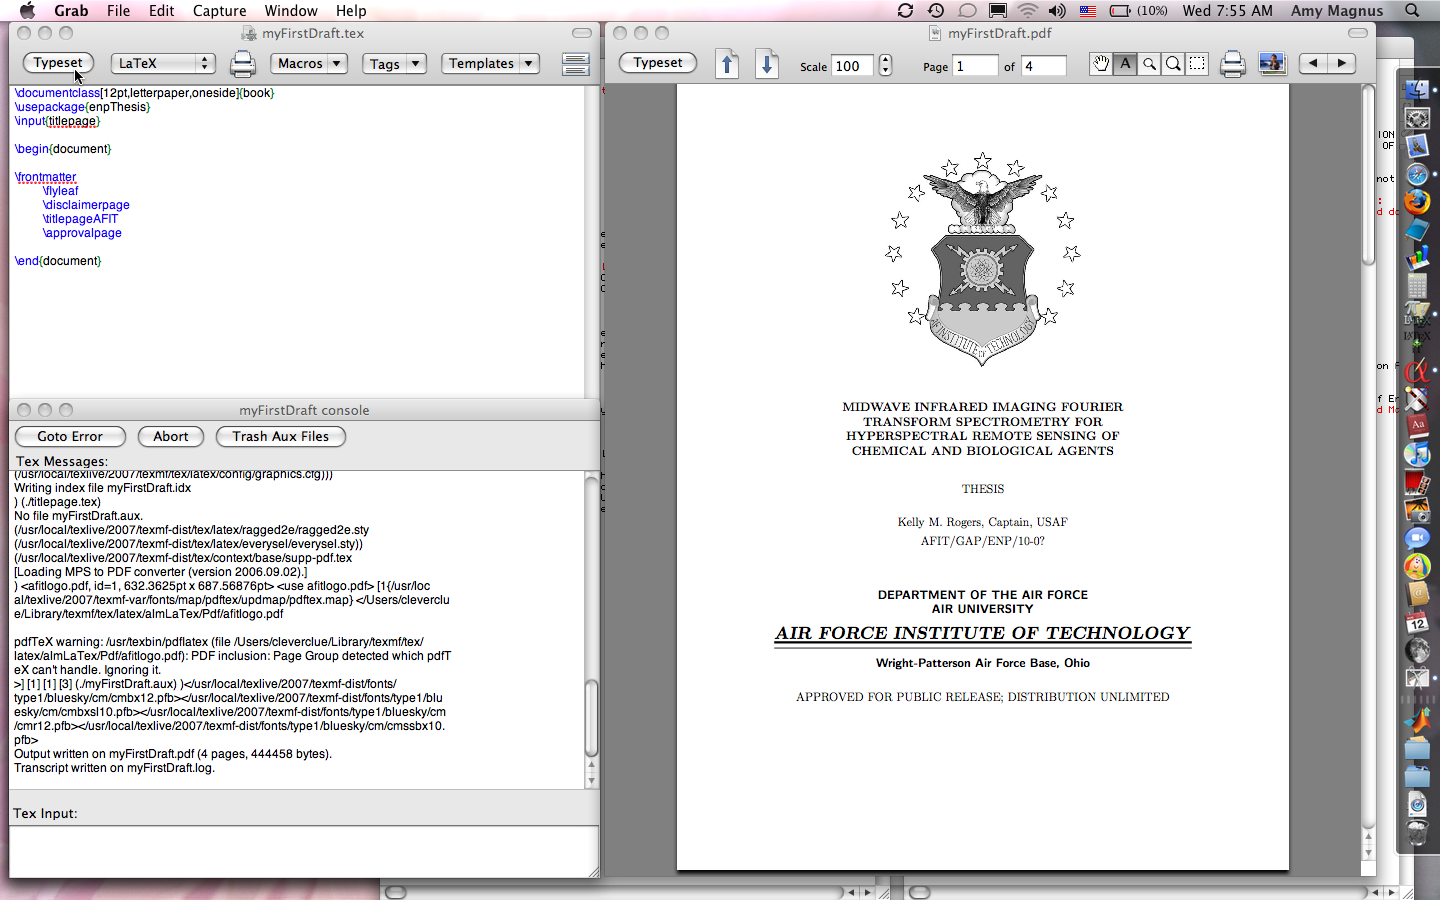
\includegraphics[width=6in]{myFlypage}
     \caption{Here we have compiled the first four page of a thesis.}
     \label{fig:myFlypage}
 \end{center}
\end{figure}
}

\newcommand{\figmyFirstAbstract}{\begin{figure}[tbp]
 \begin{center}
    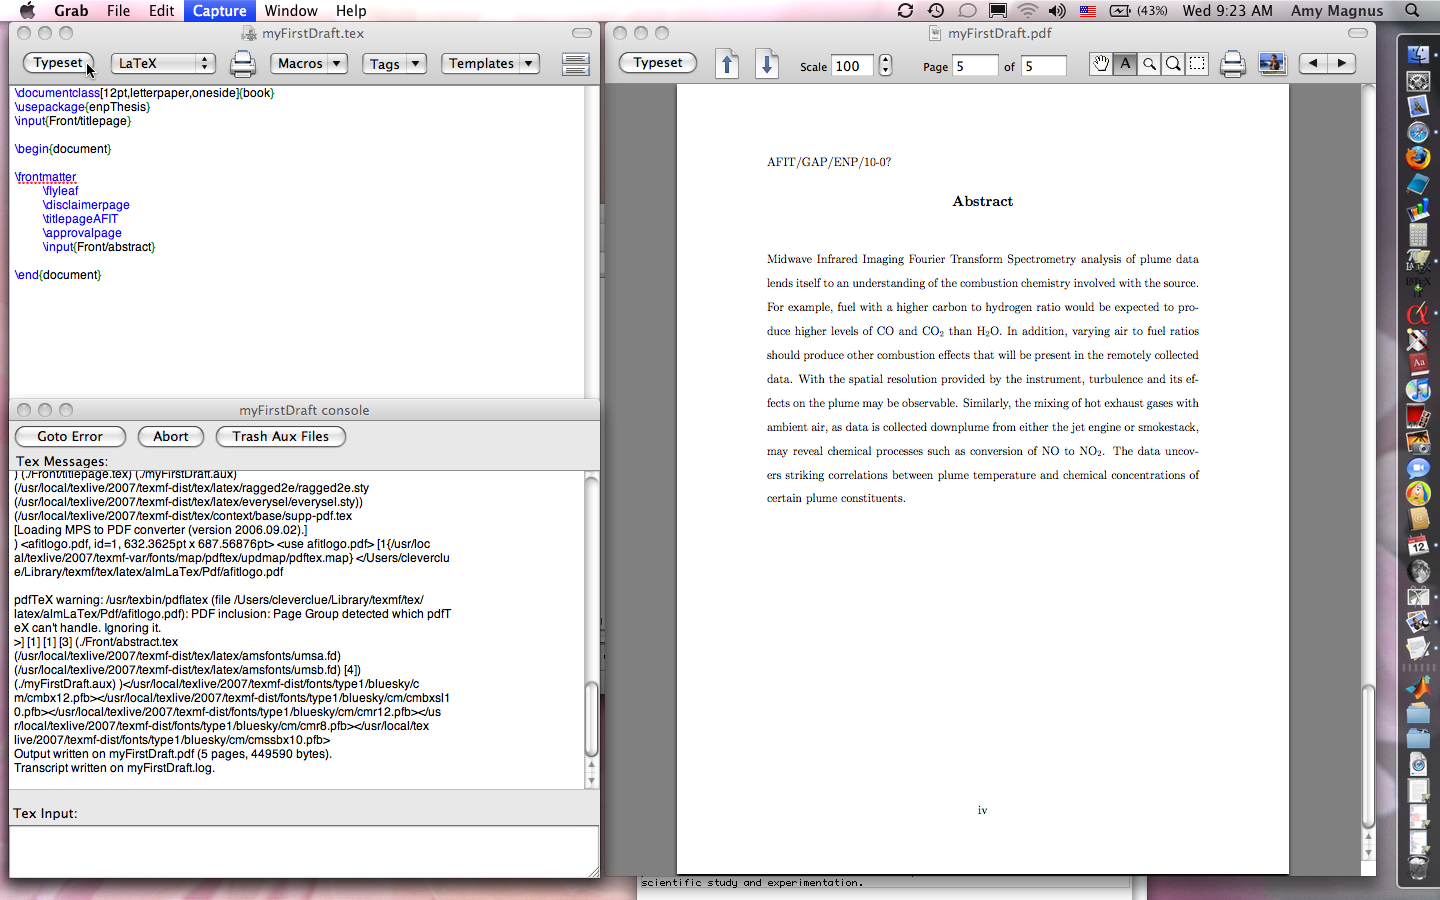
\includegraphics[width=6in]{myFirstAbstract}
     \caption{Add an abstract to the front matter of your thesis.}
     \label{fig:myFirstAbstract}
 \end{center}
\end{figure}
}

\newcommand{\figmyFigures}{\begin{figure}[tbp]
 \begin{center}
    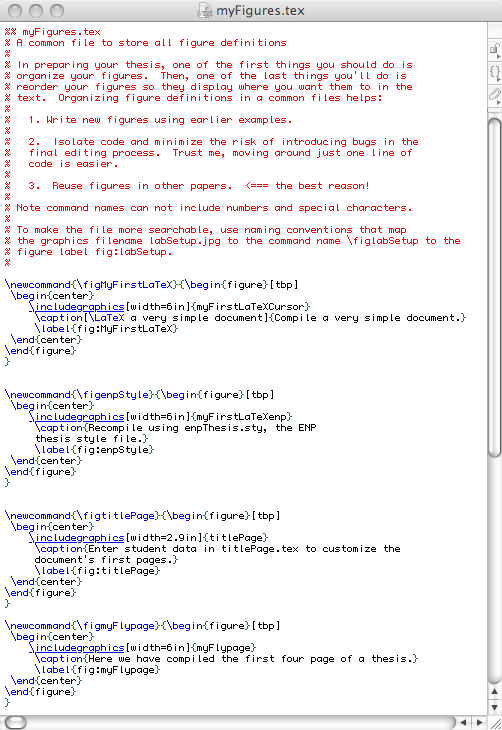
\includegraphics[width=5in]{myFigures}
     \caption{Consider defining all your figures in one file.}
     \label{fig:myFigures}
 \end{center}
\end{figure}
}


\newcommand{\figmyFirstFigures}{\begin{figure}[tbp]
 \begin{center}
    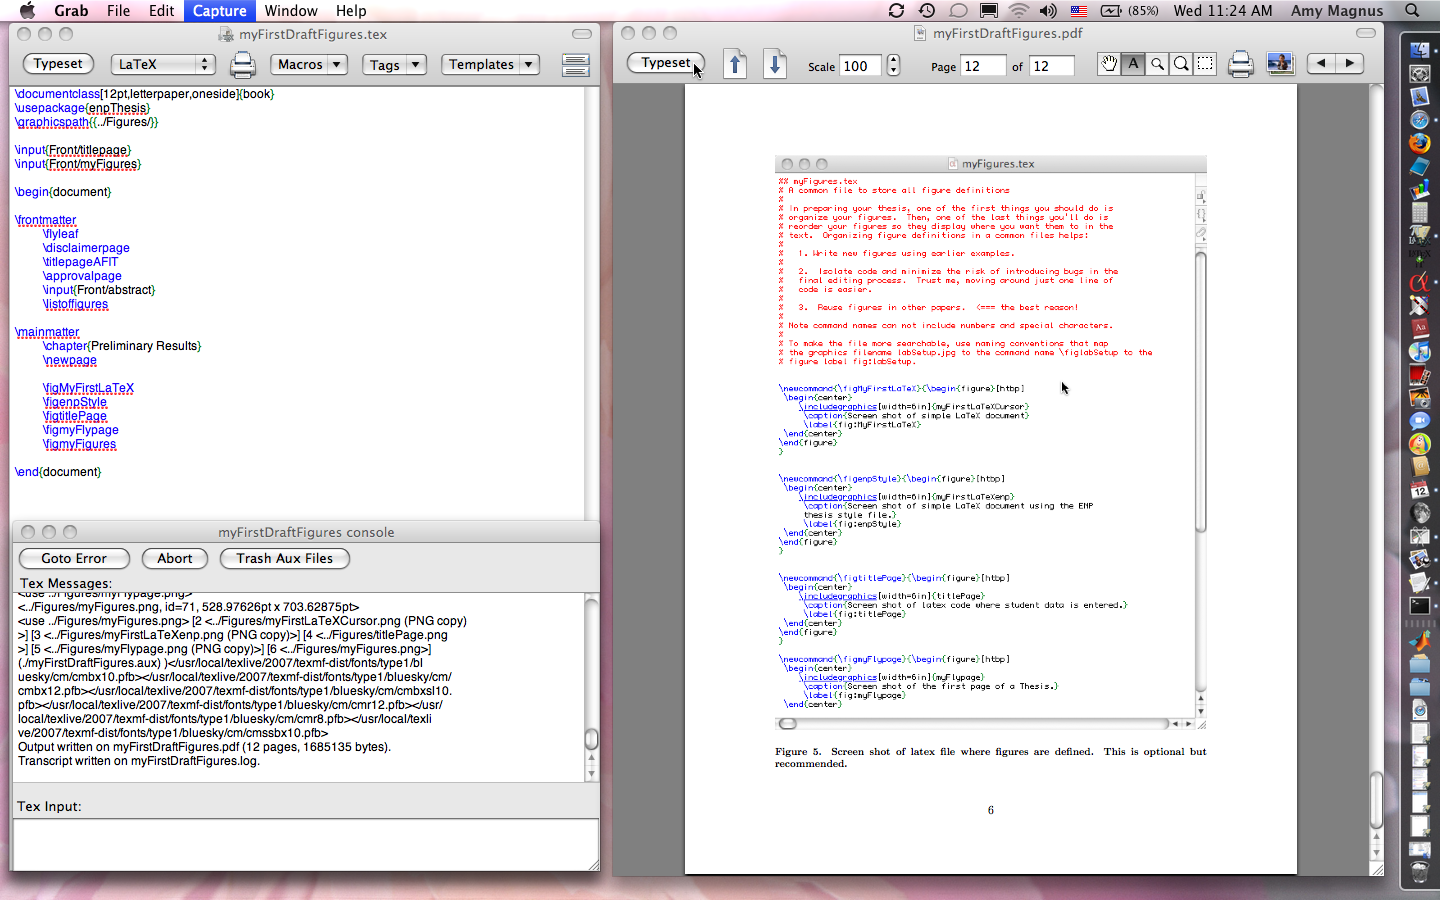
\includegraphics[width=6in]{myFirstFigures}
     \caption{Add figures in the main matter of your document; fill in
     the document around your graphics.}
     \label{fig:myFirstFigures}
 \end{center}
\end{figure}
}

\newcommand{\figmyFirstBibTeX}{\begin{figure}[tbp]
 \begin{center}
    \includegraphics[width=6in]{myFirstBibTeX}
     \caption{Add your bibliography.}
     \label{fig:myFirstBibTeX}
 \end{center}
\end{figure}
}





\begin{document}
\frontmatter
        \flyleaf                        
        \disclaimerpage                 
        \titlepageAFIT                      
        \committeepage  	
        % !TEX root = ../SteadmanThesis.tex
\begin{abstract}
Storm enhanced densities (SEDs) are ionospheric plasma enhancements that disrupt radio communications in the near-Earth space environment, degrading the Global Positioning System (GPS) and other high-frequency systems.  Accurate GPS/total electron content (TEC) correction maps produced by ionosphere models can mitigate degradations from SEDs.  An artificial SED was created and ingested via slant TEC measurements into the Global Assimilation of Ionospheric Measurements Gauss-Markov Kalman Filter Model to determine how many ground GPS receivers are needed to produce reliable GPS/TEC correction maps over the continental United States during geomagnetic storming.  It was found that 110 well-positioned GPS receivers produced the best overall TEC accuracy, although significantly improved accuracy was still achieved if 40 or more receivers were used.  It was determined that receiver positioning had a greater impact on TEC accuracy than the number of receivers.  Additionally, it was found that TEC accuracy for the SED region increased at the expense of TEC accuracy everywhere else on the map.
\end{abstract}


        \tableofcontents
        \listoffigures
\mainmatter
        \figMyFirstLaTeX
        \figafitStyle
        \figtitlePage
        \figmyFlypage
        \figmyFirstAbstract
        \figmyFigures
        \figmyFirstFigures
\end{document}
\end{verbatim}
}
\vspace{-0.1in}

From here, add text around your figures.  To produce this document, we
used the following code:

\vspace{-0.25in}
{\singlespace
\begin{verbatim}
\documentclass[12pt,letterpaper,oneside]{book}
\usepackage{afitThesis}
\graphicspath{{../Figures/}}

\input{Preamble/titlepage}
%% myFigures.tex
% A common file to store all figure definitions
%
% In preparing your thesis, one of the first things you should do is
% organize your figures.  Then, one of the last things you'll do is
% reorder your figures so they display where you want them to in the
% text.  Organizing figure definitions in a common files helps:
%
%   1. Write new figures using earlier examples.
%
%   2.  Isolate code and minimize the risk of introducing bugs in the
%   final editing process.  Trust me, moving around just one line of
%   code is easier.
%
%   3.  Reuse figures in other papers.  <=== the best reason!
%
% Note command names can not include numbers and special characters.
%
% To make the file more searchable, use naming conventions that map
% the graphics filename labSetup.jpg to the command name \figlabSetup to the
% figure label fig:labSetup.
% 

\newcommand{\figMyFirstLaTeX}{\begin{figure}[tbp]
 \begin{center}
    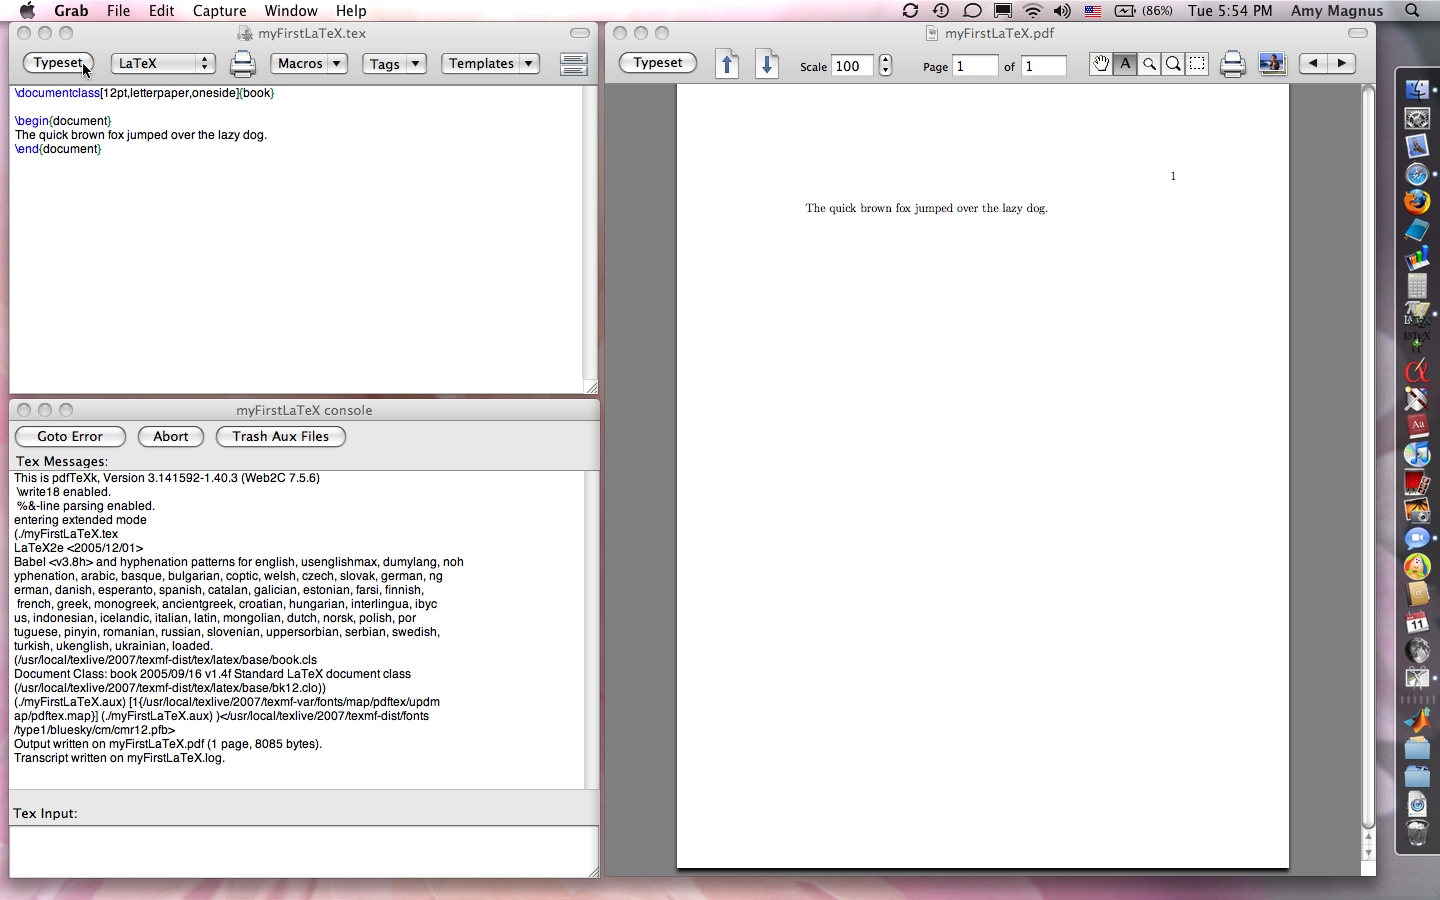
\includegraphics[width=6in]{myFirstLaTeXCursor}
     \caption[\LaTeX\ a very simple document]{Compile a very simple document.}
     \label{fig:MyFirstLaTeX}
 \end{center}
 \vspace{-0.2 in}
\end{figure}
}


\newcommand{\figafitStyle}{\begin{figure}[tbp]
 \begin{center}
    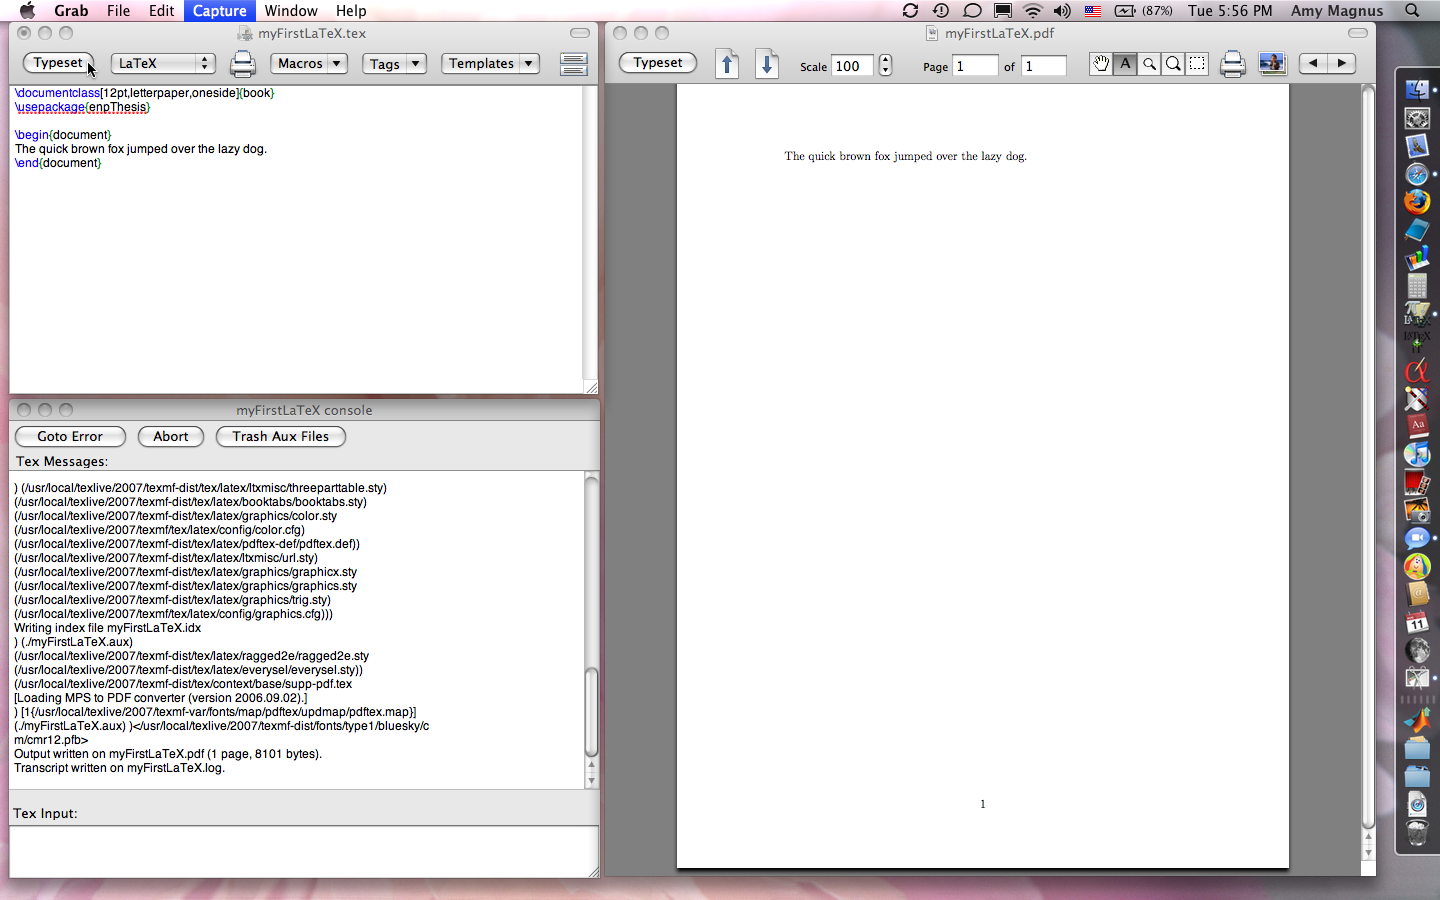
\includegraphics[width=6in]{myFirstLaTeXafit}
     \caption{Recompile using afitThesis.sty, the AFIT
     thesis style file.}
     \label{fig:afitStyle}
 \end{center}
\end{figure}
}


\newcommand{\figtitlePage}{\begin{figure}[tbp]
 \begin{center}
    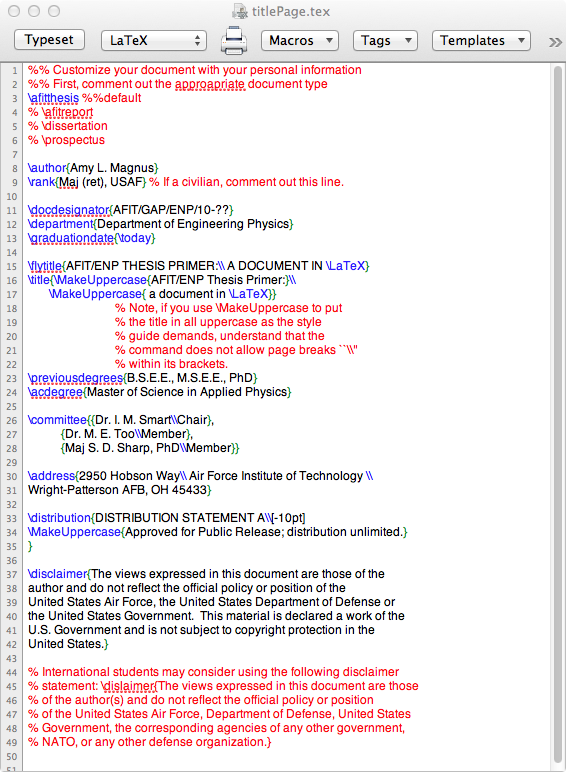
\includegraphics[width=6in]{titlePage}
     \caption{Enter student data in titlePage.tex to customize the
     document's first pages.}
     \label{fig:titlePage}
 \end{center}
\end{figure}
}

\newcommand{\figmyFlypage}{\begin{figure}[tbp]
 \begin{center}
    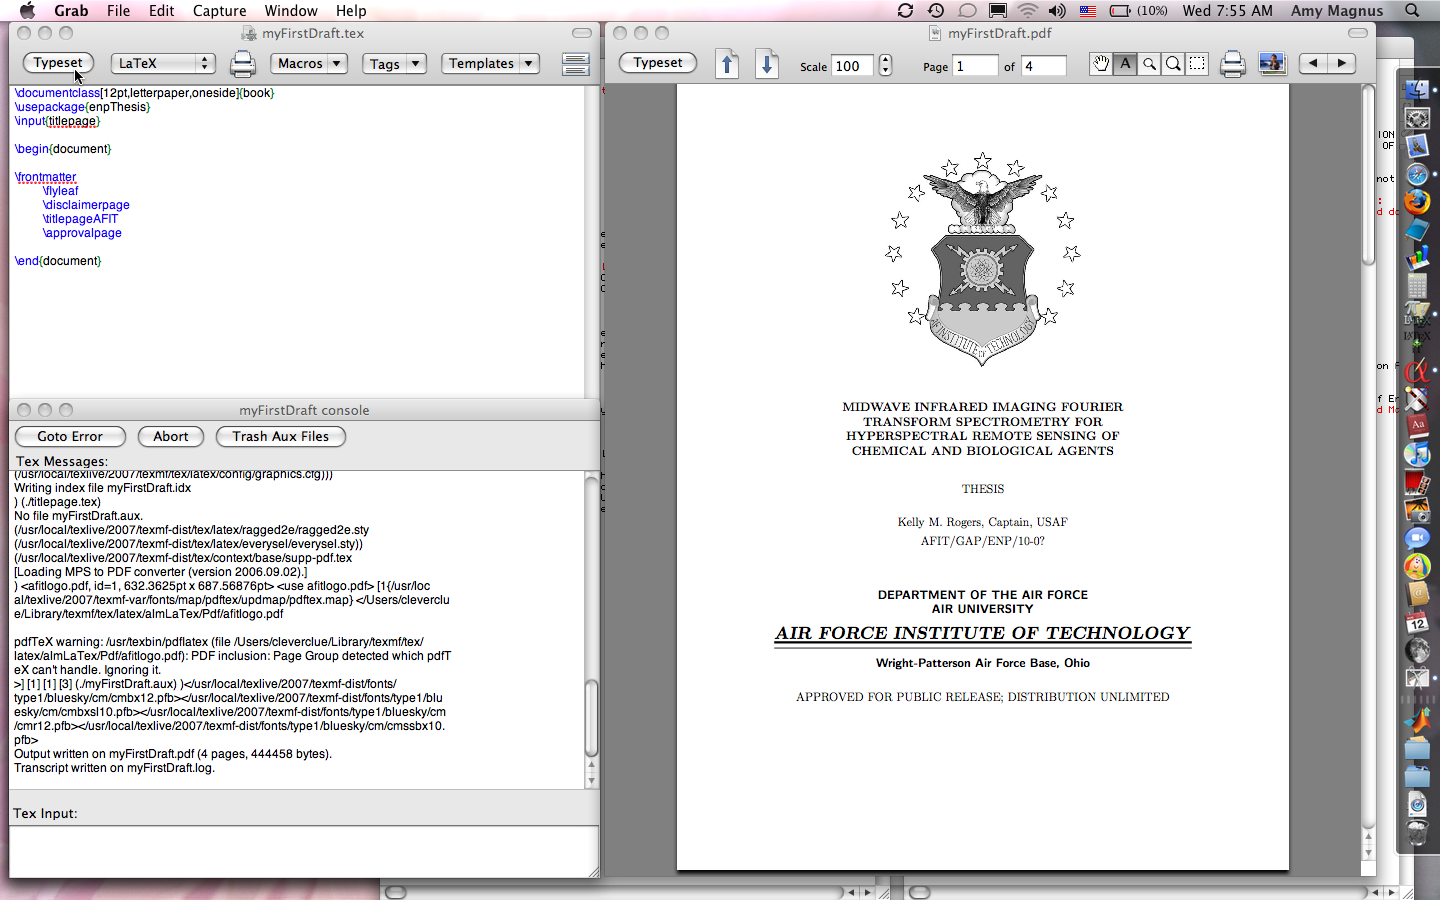
\includegraphics[width=6in]{myFlypage}
     \caption{Here we have compiled the first four page of a thesis.}
     \label{fig:myFlypage}
 \end{center}
\end{figure}
}

\newcommand{\figmyFirstAbstract}{\begin{figure}[tbp]
 \begin{center}
    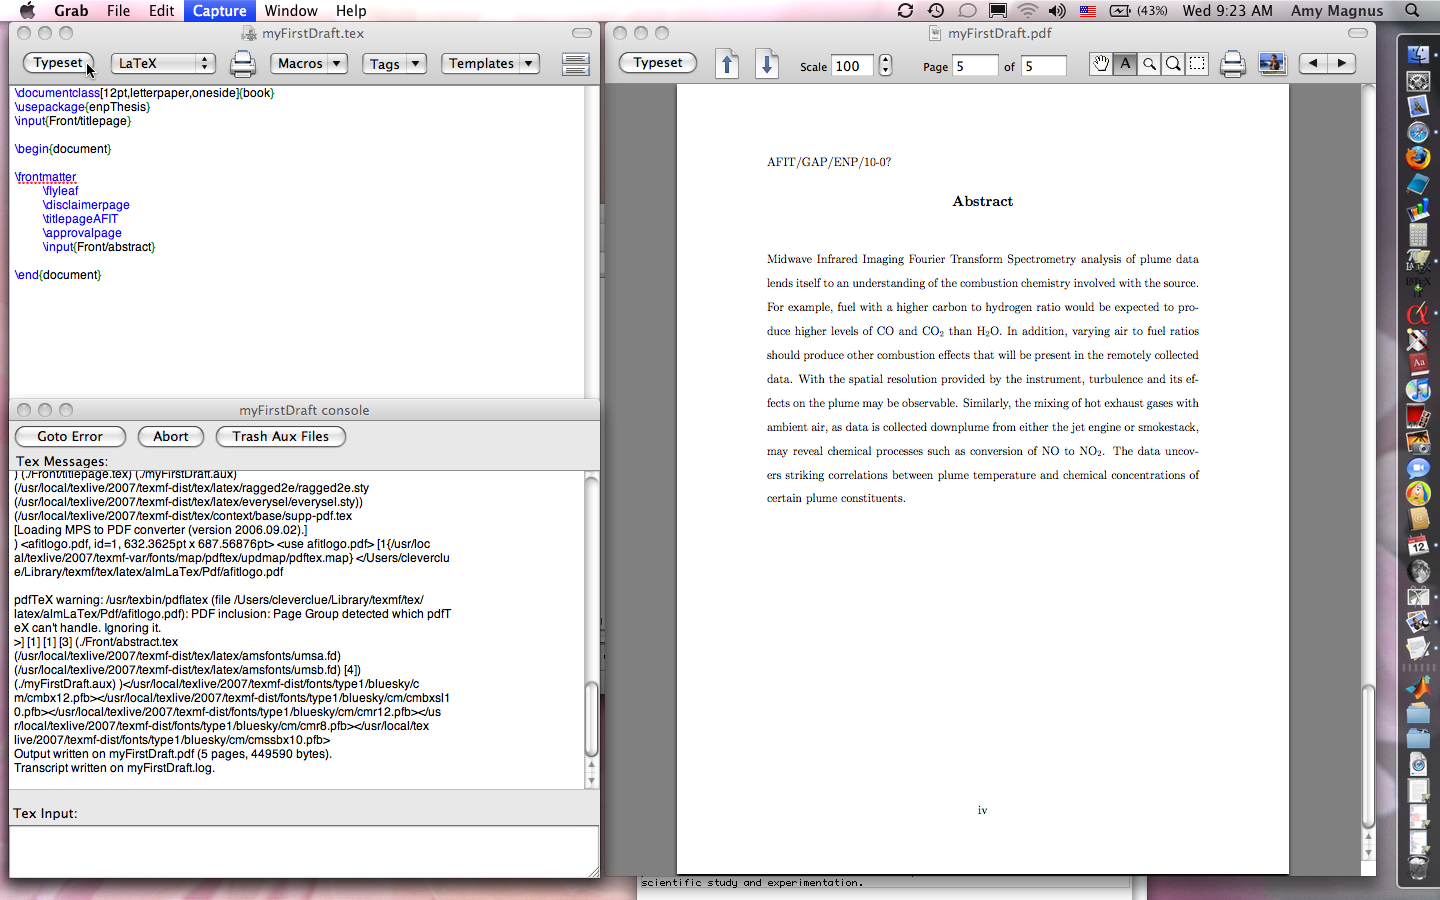
\includegraphics[width=6in]{myFirstAbstract}
     \caption{Add an abstract to the front matter of your thesis.}
     \label{fig:myFirstAbstract}
 \end{center}
\end{figure}
}

\newcommand{\figmyFigures}{\begin{figure}[tbp]
 \begin{center}
    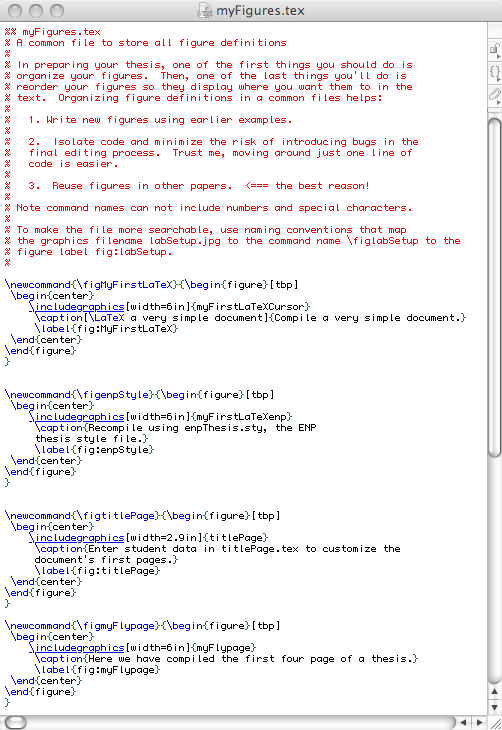
\includegraphics[width=5in]{myFigures}
     \caption{Consider defining all your figures in one file.}
     \label{fig:myFigures}
 \end{center}
\end{figure}
}


\newcommand{\figmyFirstFigures}{\begin{figure}[tbp]
 \begin{center}
    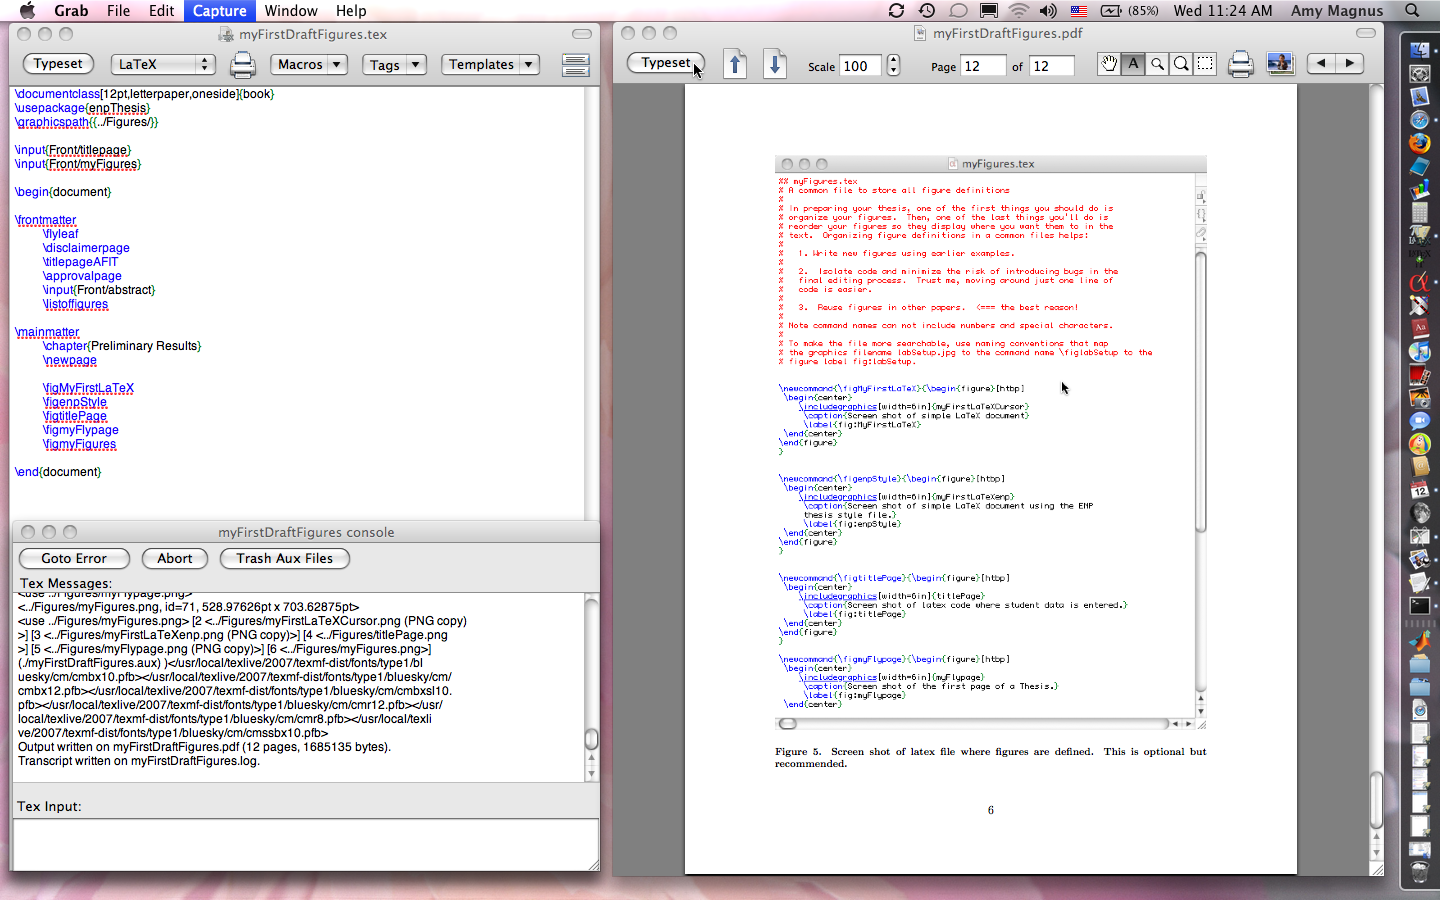
\includegraphics[width=6in]{myFirstFigures}
     \caption{Add figures in the main matter of your document; fill in
     the document around your graphics.}
     \label{fig:myFirstFigures}
 \end{center}
\end{figure}
}

\newcommand{\figmyFirstBibTeX}{\begin{figure}[tbp]
 \begin{center}
    \includegraphics[width=6in]{myFirstBibTeX}
     \caption{Add your bibliography.}
     \label{fig:myFirstBibTeX}
 \end{center}
\end{figure}
}




% define custom commands
\newcommand{\regmark}{\raisebox{5pt}{\tiny \circledR}\xspace}
\newcommand{\matlab}{\textsc{Matlab}\regmark}
\newcommand{\trademark}{\raisebox{5pt}{\tiny TM}\xspace}
\newcommand{\mca}{\texttt{Mathematica}\regmark}
\newcommand{\Latex}{\LaTeX\xspace}

% Create a new theorem style called a Corollary.
% If you don't have any, then just comment this out.
%\theoremstyle{plain} % Default
\newtheorem{cor}{Corollary}[chapter]

%Custom Commands for Student

\newcommand{\primerAddress}{{L:$\backslash$Courses$\backslash$PHYS$\backslash$LaTeX}\xspace}


\begin{document}
\frontmatter
        \flyleaf                        
        \disclaimerpage                 
        \titlepageAFIT                      
        \committeepage  
        % !TEX root = ../SteadmanThesis.tex
\begin{abstract}
Storm enhanced densities (SEDs) are ionospheric plasma enhancements that disrupt radio communications in the near-Earth space environment, degrading the Global Positioning System (GPS) and other high-frequency systems.  Accurate GPS/total electron content (TEC) correction maps produced by ionosphere models can mitigate degradations from SEDs.  An artificial SED was created and ingested via slant TEC measurements into the Global Assimilation of Ionospheric Measurements Gauss-Markov Kalman Filter Model to determine how many ground GPS receivers are needed to produce reliable GPS/TEC correction maps over the continental United States during geomagnetic storming.  It was found that 110 well-positioned GPS receivers produced the best overall TEC accuracy, although significantly improved accuracy was still achieved if 40 or more receivers were used.  It was determined that receiver positioning had a greater impact on TEC accuracy than the number of receivers.  Additionally, it was found that TEC accuracy for the SED region increased at the expense of TEC accuracy everywhere else on the map.
\end{abstract}


        \tableofcontents
        \listoffigures
        

\begin{preface}
Welcome to the world of \Latex! Learn \Latex and you can rapidly
produce papers tailored for a wide variety of publications.
When you create a digital
document\ldots whether you use a ``what you see is what you get''
(WYSIWYG) interface like Microsoft Word or a typesetting system like
\Latex\ldots you are writing a program.  In the realm of academic publishing,
\Latex helps us write a better program.   

The best reasons to write with \Latex are high quality equations,
superior graphics, and the automated generation of table of contents,
lists, and bibliographies.  We can create clean 50+ page documents
that reformat in a snap.  Additionally, due to the fact that the
\Latex typesetting system was written by and for academics, many
of its tools are free and run on Microsoft Windows, Mac OS X, and
Linux.

So let's get started.  Download a \Latex distribution for 
your computer platform, set up your editor and compiler and we'll get 
cracking.  
\end{preface}



\mainmatter
        \chapter{The First Steps}
                Take the first steps in writing your thesis using the simple programs
described in this chapter as a guide.  The source code and support files can be
found on the student drive \primerAddress.  With a
current \Latex distribution\footnote{\Latex distributions update
annually in June.  As of June 2014, the current \Latex
distributions are MiKTeX 2.9 for Windows, TeX Live 2014 for Linux, and
MacTeX 2014 for Macintosh.}, you will be able to compile these programs
without hiccup.

The directory tree below provides a recommended file structure
for the papers generated in your research.  Directories follow ``$>$'' signs; 
standared\ files are
specified in parentheses. 
{\singlespace
\begin{lstlisting}
> myLatexDocuments
  >> afitStyleFiles (afitThesis.sty)
  >> Figures (afitlogo.pdf, afitlogo.eps)
  >> Thesis  (myThesis.tex)
     >>> Preamble (titlePage.tex,myFigures.tex)
     >>> Front (abstract.tex)
     >>> Chapter01 (sectionOne,sectionTwo,...)
     >>> Chapter02 
     . . .
     >>> Appendix01
     . . .
  >> Archived Draft of Thesis 
  >> Archived Perspectus 
  >> Paper One
  >> Paper Two
\end{lstlisting}
} \noindent In a parent directory, create three directories
``afitStyleFiles'', ``Figures'', and ``Thesis''.  Place your graphics
(such as afitlogo.pdf) in the directory Figures, your \Latex style
files (afitThesis.sty, sf298.sty, sf298.dtx, and sf298.ins) in
afitStyleFiles, and the latex code for your thesis document in Thesis.
Organized in this way, the files in the Figures directory and the
afitStyleFiles directory can be used by your thesis, perspectus, archived drafts,
and other publications.  Typically, graphics account for most of the
memory taken up by a digital document, and this efficiency in
sharing saves significant disk space.



		
                \figMyFirstLaTeX
                \section{\Latex a simple document}
                To compile a LaTex document, start simple with the code listed 
below.  Store the code as a .tex file in your
Thesis directory. Then compile the code to test the set up of your \Latex 
distribution and compiler\footnote{Popular compilers include TeXworks 
and TeXShop.}.  Figure~\ref{fig:MyFirstLaTeX} provides a screen
shot of the typeset document with its compilation aids.

 {\singlespace   
 \begin{verbatim}
\documentclass[12pt,letterpaper,oneside]{book}
 
\begin{document}
The quick brown fox jumped over the lazy dog.
\end{document}
\end{verbatim}
} 
\noindent The code has two parts: the preamble and the body.  The
preamble establishes the default formatting for the document; the body
holds the content.  The preamble starts with a {\bf $\backslash$documentclass}
declaration and ends at the {\bf $\backslash$begin\{document\}}
command. The {body} is placed in between the {\bf
$\backslash$begin\{document\}} and {\bf $\backslash$end\{document\}}
commands. 

In the preamble of this first document, Here we have selected a one
sided, 12-pt font book format.  In the body, let us enter a short
phrase---just to get a feel for how content is added---that includes 
all characters in the Roman alphabet.
    
   
%Other formats include article, report, memoir The body contains the
%actual content.


		

                \figafitStyle
                \section{Add a style file}
                Next, we add the style file afitThesis.sty to the preamble and
recompile.  The style file implements the AFIT thesis format and is
added via the command {\bf $\backslash$usepackage}.

\vspace{-0.3in}
{\singlespace
\begin{verbatim}
\documentclass[12pt,letterpaper,oneside]{book}
\usepackage{../afitStyleFiles/afitThesis}

\begin{document}
The quick brown fox jumped over the lazy dog.
\end{document}
\end{verbatim}
} \noindent Note the resulting changes to the document in
Figure~\ref{fig:afitStyle}.  Some adjustments are immediately apparent:
The margins have changed and a page number is now located at the
bottom of the page.
    

		

                \figtitlePage
                \section{Add the front matter}
                The style file {\em afitThesis.sty} contains code that generates the
first, standardized pages of the thesis document.  Theses pages are the
flyleaf, disclaimer page, the title page, and the committee page.  For
each thesis, we customize these four pages by editing a tex file
called {\em titlePage.tex}.  The customizable items for a thesis are:

\vspace{-0.15in}
\begin{tabular}{p{2.2in}p{4in}}
    \begin{itemize}\itemsep-10pt
	    \item Author
	    \item Rank
	    \item Graduation Date
	    \item Document Designator
	    \item Flypage title
	    \item Title
     \end{itemize} &
    \begin{itemize}\itemsep-10pt
	    \item Previous degrees
	    \item Academic degree upon AFIT graduation
	    \item Committee membership
	    \item Department granting your degree
	    \item School address
	    \item Distribution statement
	    \item Disclaimer
     \end{itemize} 
\end{tabular}

\noindent Add this information to {\em titlePage.tex} as you obtain
it.  One item to include as soon as possible is the distribution
statement; ask your advisor which distribution statement is
appropriate for your draft document.
    
If your document is something other than a thesis, you can set a flag at
the beginning of {\em titlePage.tex}.  Use the $\%$ symbol to comment
out unused flags and remove the $\%$ from the line of the
appropriate flag.  In this way, the correct flag will execute at
compilation.  The available flags correspond to the following
documents:

\vspace{-0.3in}
{\singlespace
\begin{center}
\begin{tabular}{|l|l|}
    \hline
    \bf Document & \bf Flag\\
    \hline
    Thesis & {\bf $\backslash$afitthesis}  \\
    Report & {\bf $\backslash$afitreport} \\
    Dissertation & {\bf $\backslash$dissertation} \\
    Prospectus & {\bf $\backslash$prospectus}\\
    \hline
\end{tabular}
\end{center}}

Once you customize the {\em titlePage.tex} file, we can typeset
the first four pages of an AFIT thesis: the flypage, the disclaimer
page, the title page and the committee page. 

We must add a few lines to our typesetting program.  Within the
document environment, we list the first four pages (See line 7-11)
under front matter.  The flypage includes our first graphic---the AFIT
logo---so we provide a path to our figures by using the {\bf
$\backslash$graphicspath} command\footnote{Note the double brackets
used in the graphicspath command; they are necessary for the command
to execute properly with some compilers.} in the preamble.  Note line
3 below where we set the path.  The {\em titlePage.tex} provides
customization, not content, so it is called in the preamble;
call the file by using the command {\bf $\backslash$input} as in line
4 of the code below.  In all, we have added seven lines of code to our
short program to create a four page document.

\vspace{-0.25in}
{\singlespace
\begin{verbatim}
\documentclass[12pt,letterpaper,oneside]{book}
\usepackage{afitThesis}
\graphicspath{{..\Figures}}
\input{Preamble/titlepage}

\begin{document}
\frontmatter
        \flyleaf                        
        \disclaimerpage                 
        \titlepageAFIT                      
        \committeepage  	
\end{document}
\end{verbatim}
}


                \figmyFlypage
                
\noindent The next section to add to the front matter is an abstract.
Create a file {\em abstract.tex} and place the text for the abstract
between the commands {\bf $\backslash$begin\{abstract\}} and {\bf
$\backslash$end\{abstract\}} as below.

\vspace{-0.3in}
{\singlespace
\begin{verbatim}
\begin{abstract}
    Midwave Infrared Imaging Fourier Transform Spectrometry analysis of
    plume data lends itself to an understanding of the combustion
    chemistry involved with the source. ...
\end{abstract}
\end{verbatim}
}

Above, we use a construct called an environment.  There are several
enviroments: figure, itemize,
verbatim, quote, equation to name a few.  \Latex friendly editors will
help you build these environments.  The abstract environment is
actually a customized environment created in the {\em afitThesis.sty}
file; thus, it will not be found in the common \Latex literature or
tools; but, as you can see above, it is simple to implement.



                \figmyFirstAbstract
                Other common items that can be added to the front matter are
acknowledgements, the table of contents and lists of figures and
tables.  The acknowledgements can be added in the same manner as the
abstract; use the environment commands for the
Acknowledgement: {\bf $\backslash$begin\{acknowledgement\}} and {\bf
$\backslash$end\{acknowledgement\}}.  The table of contents and other lists
build automatically as you add sections, figures, and tables and are placed
in the front matter using the commands below.  

\vspace{-0.3in} {\singlespace
\begin{verbatim}
\frontmatter
        \flyleaf                        
        \disclaimerpage                 
        \titlepageAFIT                      
        \committeepage
        % !TEX root = ../SteadmanThesis.tex
\begin{abstract}
Storm enhanced densities (SEDs) are ionospheric plasma enhancements that disrupt radio communications in the near-Earth space environment, degrading the Global Positioning System (GPS) and other high-frequency systems.  Accurate GPS/total electron content (TEC) correction maps produced by ionosphere models can mitigate degradations from SEDs.  An artificial SED was created and ingested via slant TEC measurements into the Global Assimilation of Ionospheric Measurements Gauss-Markov Kalman Filter Model to determine how many ground GPS receivers are needed to produce reliable GPS/TEC correction maps over the continental United States during geomagnetic storming.  It was found that 110 well-positioned GPS receivers produced the best overall TEC accuracy, although significantly improved accuracy was still achieved if 40 or more receivers were used.  It was determined that receiver positioning had a greater impact on TEC accuracy than the number of receivers.  Additionally, it was found that TEC accuracy for the SED region increased at the expense of TEC accuracy everywhere else on the map.
\end{abstract}


        \input{Front/acknowledgement}
        \tableofcontents
        \listoffigures
        \listoftables
\end{verbatim}
}

\noindent The order follows the AFIT style guide\cite{AFITStyle}.  The {\em
afitThesis.sty} defines additional environments and lists.  We
will describe how to implement those items in the next chapter.
For now, we will simply keep the abstract and perhaps the list of
figures in our front matter as we move on to the
main body of the thesis.






                \section{Add figures to the main matter and start writing}
                \figmyFigures
                
To concentrate on your research, consider organizing your figures
first.  Build the document around your figures, and you will be able
to concentrate on the story of your contribution---not the work that
has gone on before.  

To organizing your figures, it is helpful to define them in a
common file.  See {\em myFigures.tex} depicted in
Figure~\ref{fig:myFigures} and stored in the Preamble subdirectory.
In this way, you may:
    \begin{itemize}
      \item Readily write new figures using earlier examples. 
      
      \item  Isolate code and minimize the risk of introducing bugs in the
      final editing process.  Moving around one line of
      code is easy and safe.
      
      \item Standardize figures without having to locate them 
      throughout the document.
      
      \item  Reuse figures in other papers.  $\leftarrow$ The best reason!
    \end{itemize}
        
\noindent In {\em myFigures.tex}, use {\bf
$\backslash${newcommand}} to define a command for each figure as
below:

{\vspace{-.30in}}
{\singlespace
\begin{verbatim}
\newcommand{\figmyFigures}{
    \begin{figure}[htbp]
        \begin{center}
             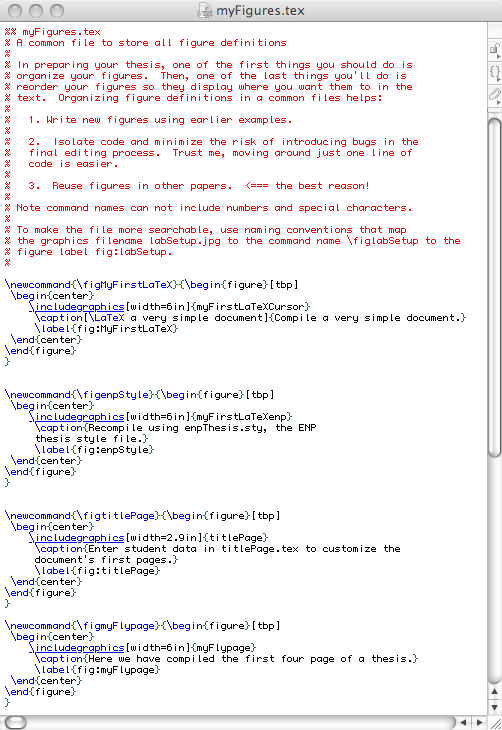
\includegraphics[width=6in]{myFigures}
             \caption{A sample tex file where figures are defined.}
             \label{fig:myFigures}
        \end{center}
    \end{figure}
}
\end{verbatim}}
    
\noindent For a command, chose a naming convention that
intuitively links the command to the graphic file and the figure
label.  For example, above we have defined a command {\bf
$\backslash${figmyFigures}} to position a figure containing graphic
myFigures.png.  Note command names cannot include numbers or special
characters.



                \figmyFirstFigures
                
Now, in the preamble of your code, input {\em myFigures.tex} in the
same manner as you input {\em titlepage.tex}.  Now we are ready to add
the main body of the thesis.  Initiate the main body of your document
by calling the {\bf$\backslash$mainmatter} command.  Next, call the
figures that you have defined and compile.  Note, once you add a
chapter, you can remove {\bf$\backslash$thispagestyle\{plain\}} which
precedes the {\bf$\backslash$mainmatter} command.

\vspace{-0.3in}
{\singlespace
\begin{verbatim}
\documentclass[12pt,letterpaper,oneside]{book}
\usepackage{afitThesis}
\graphicspath{{..\Figures}}
\input{Preamble/titlepage}
%% myFigures.tex
% A common file to store all figure definitions
%
% In preparing your thesis, one of the first things you should do is
% organize your figures.  Then, one of the last things you'll do is
% reorder your figures so they display where you want them to in the
% text.  Organizing figure definitions in a common files helps:
%
%   1. Write new figures using earlier examples.
%
%   2.  Isolate code and minimize the risk of introducing bugs in the
%   final editing process.  Trust me, moving around just one line of
%   code is easier.
%
%   3.  Reuse figures in other papers.  <=== the best reason!
%
% Note command names can not include numbers and special characters.
%
% To make the file more searchable, use naming conventions that map
% the graphics filename labSetup.jpg to the command name \figlabSetup to the
% figure label fig:labSetup.
% 

\newcommand{\figMyFirstLaTeX}{\begin{figure}[tbp]
 \begin{center}
    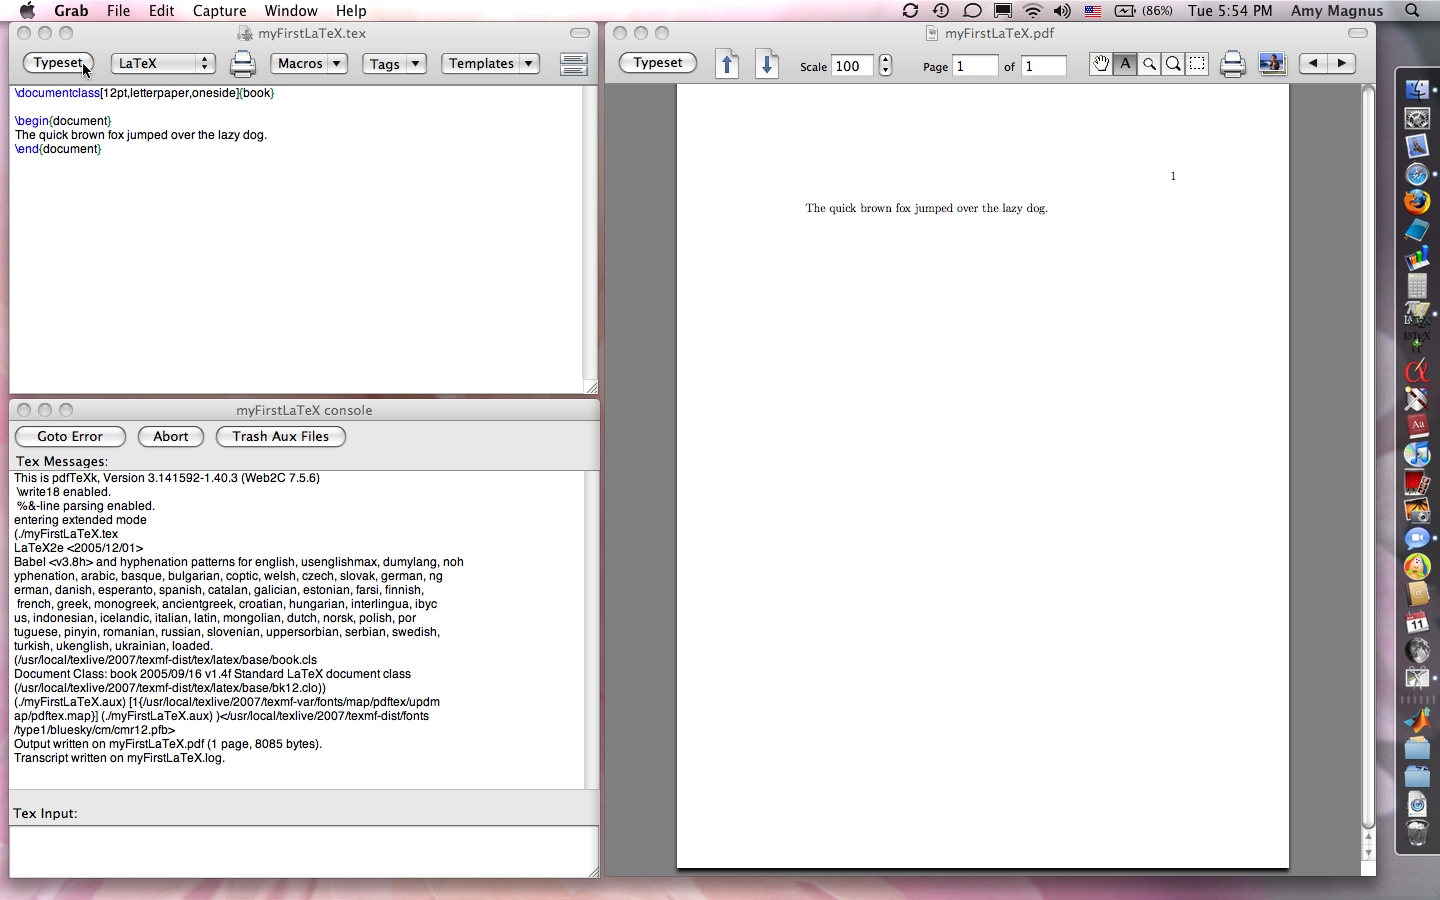
\includegraphics[width=6in]{myFirstLaTeXCursor}
     \caption[\LaTeX\ a very simple document]{Compile a very simple document.}
     \label{fig:MyFirstLaTeX}
 \end{center}
 \vspace{-0.2 in}
\end{figure}
}


\newcommand{\figafitStyle}{\begin{figure}[tbp]
 \begin{center}
    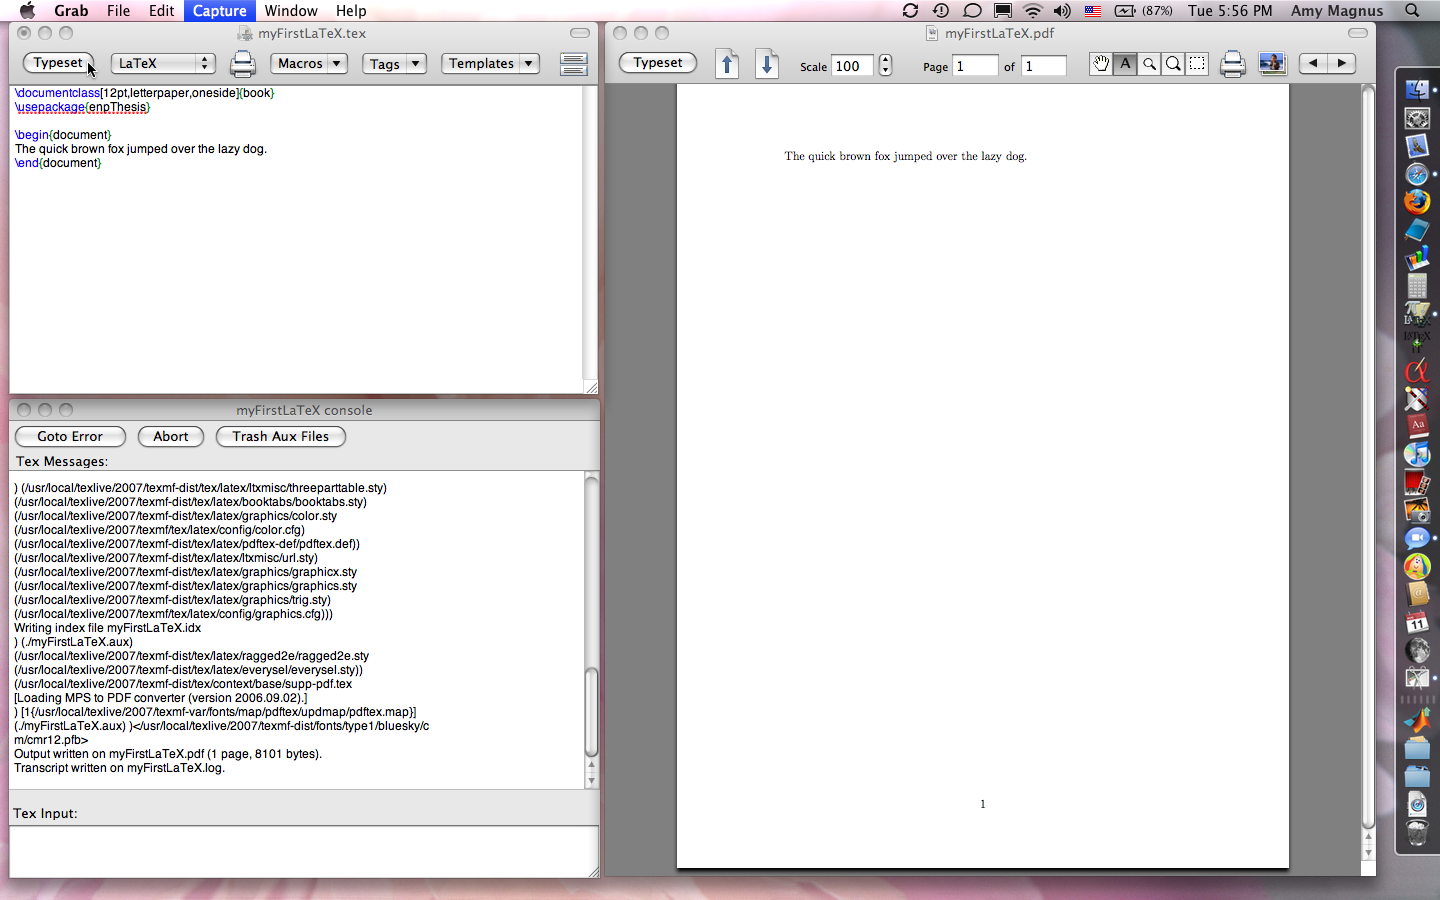
\includegraphics[width=6in]{myFirstLaTeXafit}
     \caption{Recompile using afitThesis.sty, the AFIT
     thesis style file.}
     \label{fig:afitStyle}
 \end{center}
\end{figure}
}


\newcommand{\figtitlePage}{\begin{figure}[tbp]
 \begin{center}
    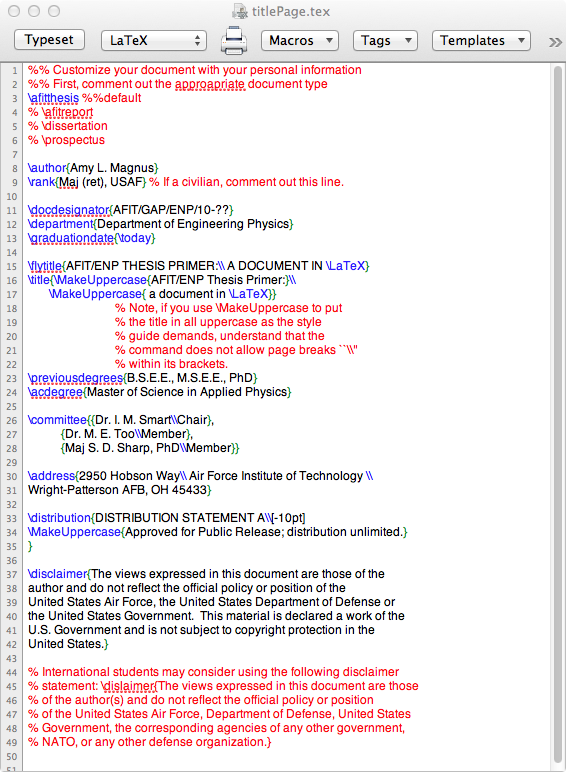
\includegraphics[width=6in]{titlePage}
     \caption{Enter student data in titlePage.tex to customize the
     document's first pages.}
     \label{fig:titlePage}
 \end{center}
\end{figure}
}

\newcommand{\figmyFlypage}{\begin{figure}[tbp]
 \begin{center}
    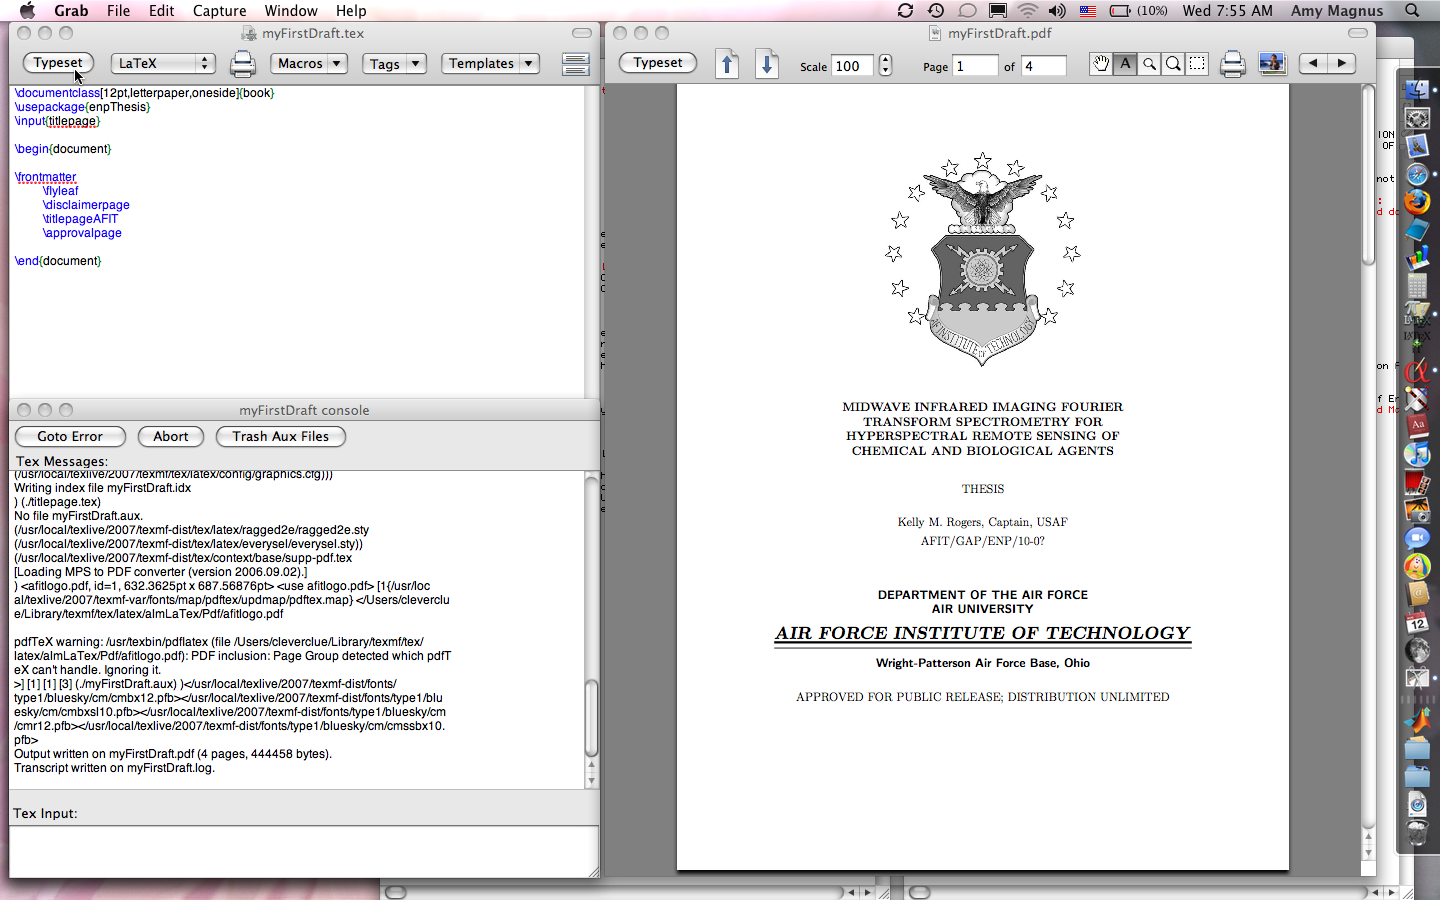
\includegraphics[width=6in]{myFlypage}
     \caption{Here we have compiled the first four page of a thesis.}
     \label{fig:myFlypage}
 \end{center}
\end{figure}
}

\newcommand{\figmyFirstAbstract}{\begin{figure}[tbp]
 \begin{center}
    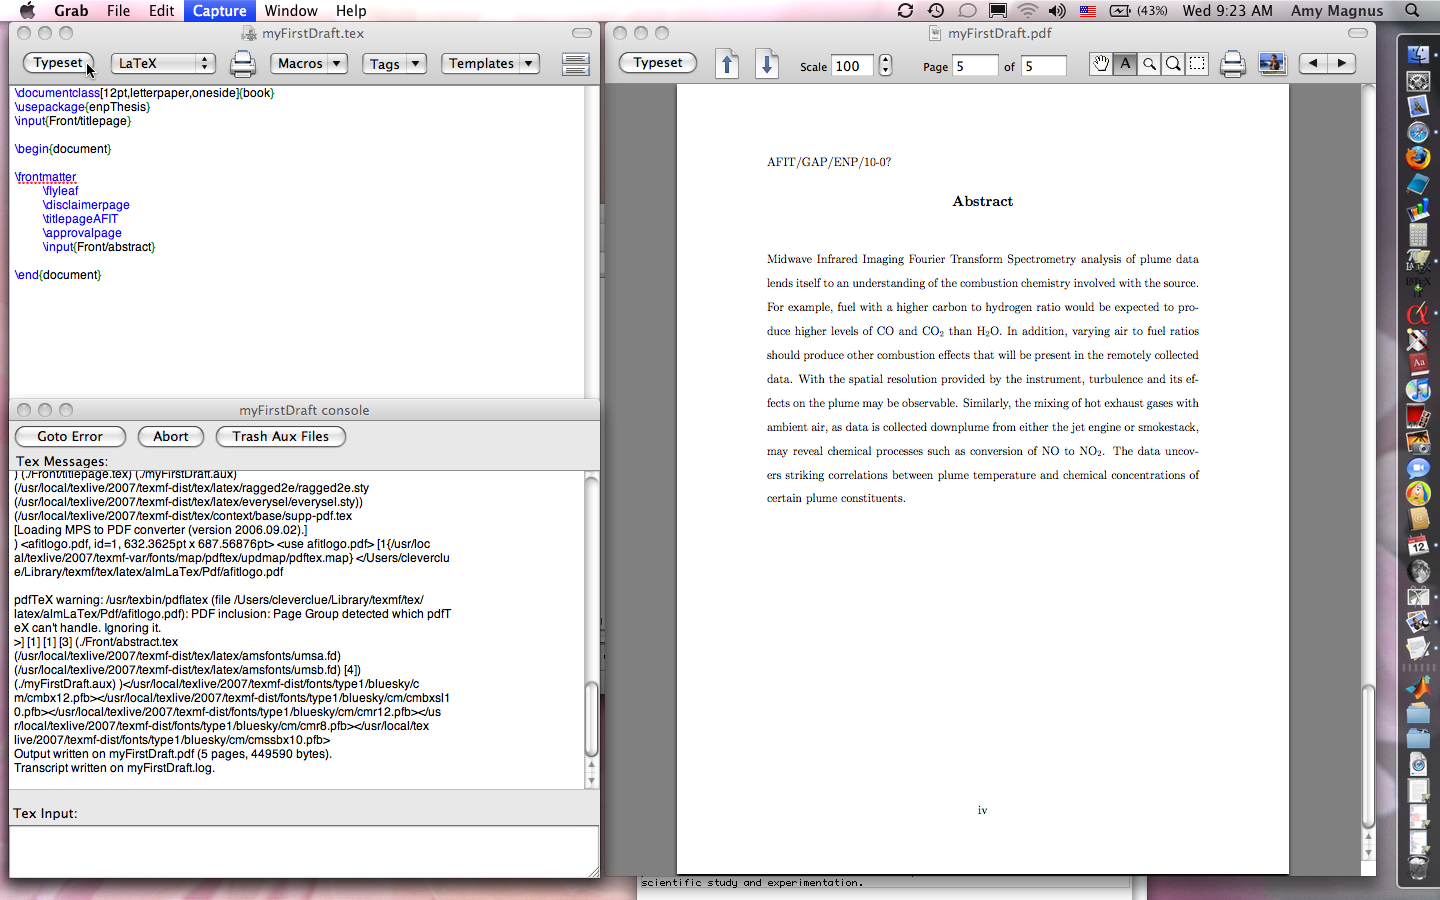
\includegraphics[width=6in]{myFirstAbstract}
     \caption{Add an abstract to the front matter of your thesis.}
     \label{fig:myFirstAbstract}
 \end{center}
\end{figure}
}

\newcommand{\figmyFigures}{\begin{figure}[tbp]
 \begin{center}
    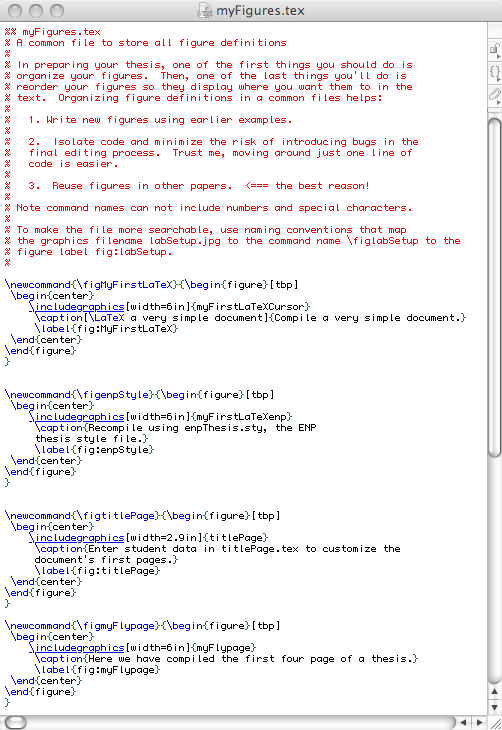
\includegraphics[width=5in]{myFigures}
     \caption{Consider defining all your figures in one file.}
     \label{fig:myFigures}
 \end{center}
\end{figure}
}


\newcommand{\figmyFirstFigures}{\begin{figure}[tbp]
 \begin{center}
    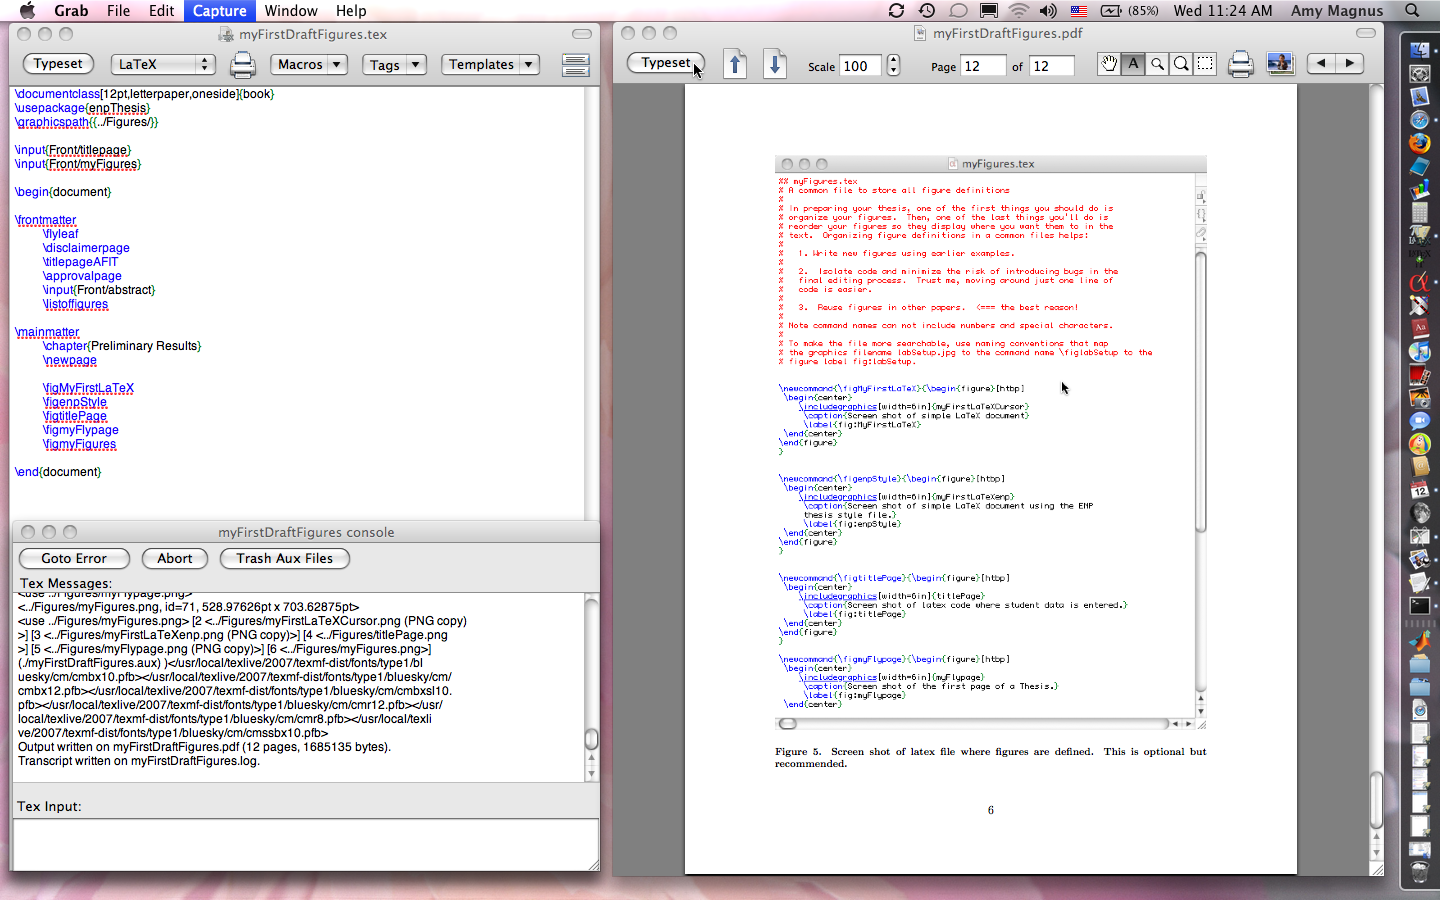
\includegraphics[width=6in]{myFirstFigures}
     \caption{Add figures in the main matter of your document; fill in
     the document around your graphics.}
     \label{fig:myFirstFigures}
 \end{center}
\end{figure}
}

\newcommand{\figmyFirstBibTeX}{\begin{figure}[tbp]
 \begin{center}
    \includegraphics[width=6in]{myFirstBibTeX}
     \caption{Add your bibliography.}
     \label{fig:myFirstBibTeX}
 \end{center}
\end{figure}
}





\begin{document}
\frontmatter
        \flyleaf                        
        \disclaimerpage                 
        \titlepageAFIT                      
        \committeepage  	
        % !TEX root = ../SteadmanThesis.tex
\begin{abstract}
Storm enhanced densities (SEDs) are ionospheric plasma enhancements that disrupt radio communications in the near-Earth space environment, degrading the Global Positioning System (GPS) and other high-frequency systems.  Accurate GPS/total electron content (TEC) correction maps produced by ionosphere models can mitigate degradations from SEDs.  An artificial SED was created and ingested via slant TEC measurements into the Global Assimilation of Ionospheric Measurements Gauss-Markov Kalman Filter Model to determine how many ground GPS receivers are needed to produce reliable GPS/TEC correction maps over the continental United States during geomagnetic storming.  It was found that 110 well-positioned GPS receivers produced the best overall TEC accuracy, although significantly improved accuracy was still achieved if 40 or more receivers were used.  It was determined that receiver positioning had a greater impact on TEC accuracy than the number of receivers.  Additionally, it was found that TEC accuracy for the SED region increased at the expense of TEC accuracy everywhere else on the map.
\end{abstract}


        \tableofcontents
        \listoffigures
\mainmatter
        \figMyFirstLaTeX
        \figafitStyle
        \figtitlePage
        \figmyFlypage
        \figmyFirstAbstract
        \figmyFigures
        \figmyFirstFigures
\end{document}
\end{verbatim}
}
\vspace{-0.1in}

From here, add text around your figures.  To produce this document, we
used the following code:

\vspace{-0.25in}
{\singlespace
\begin{verbatim}
\documentclass[12pt,letterpaper,oneside]{book}
\usepackage{afitThesis}
\graphicspath{{../Figures/}}

\input{Preamble/titlepage}
%% myFigures.tex
% A common file to store all figure definitions
%
% In preparing your thesis, one of the first things you should do is
% organize your figures.  Then, one of the last things you'll do is
% reorder your figures so they display where you want them to in the
% text.  Organizing figure definitions in a common files helps:
%
%   1. Write new figures using earlier examples.
%
%   2.  Isolate code and minimize the risk of introducing bugs in the
%   final editing process.  Trust me, moving around just one line of
%   code is easier.
%
%   3.  Reuse figures in other papers.  <=== the best reason!
%
% Note command names can not include numbers and special characters.
%
% To make the file more searchable, use naming conventions that map
% the graphics filename labSetup.jpg to the command name \figlabSetup to the
% figure label fig:labSetup.
% 

\newcommand{\figMyFirstLaTeX}{\begin{figure}[tbp]
 \begin{center}
    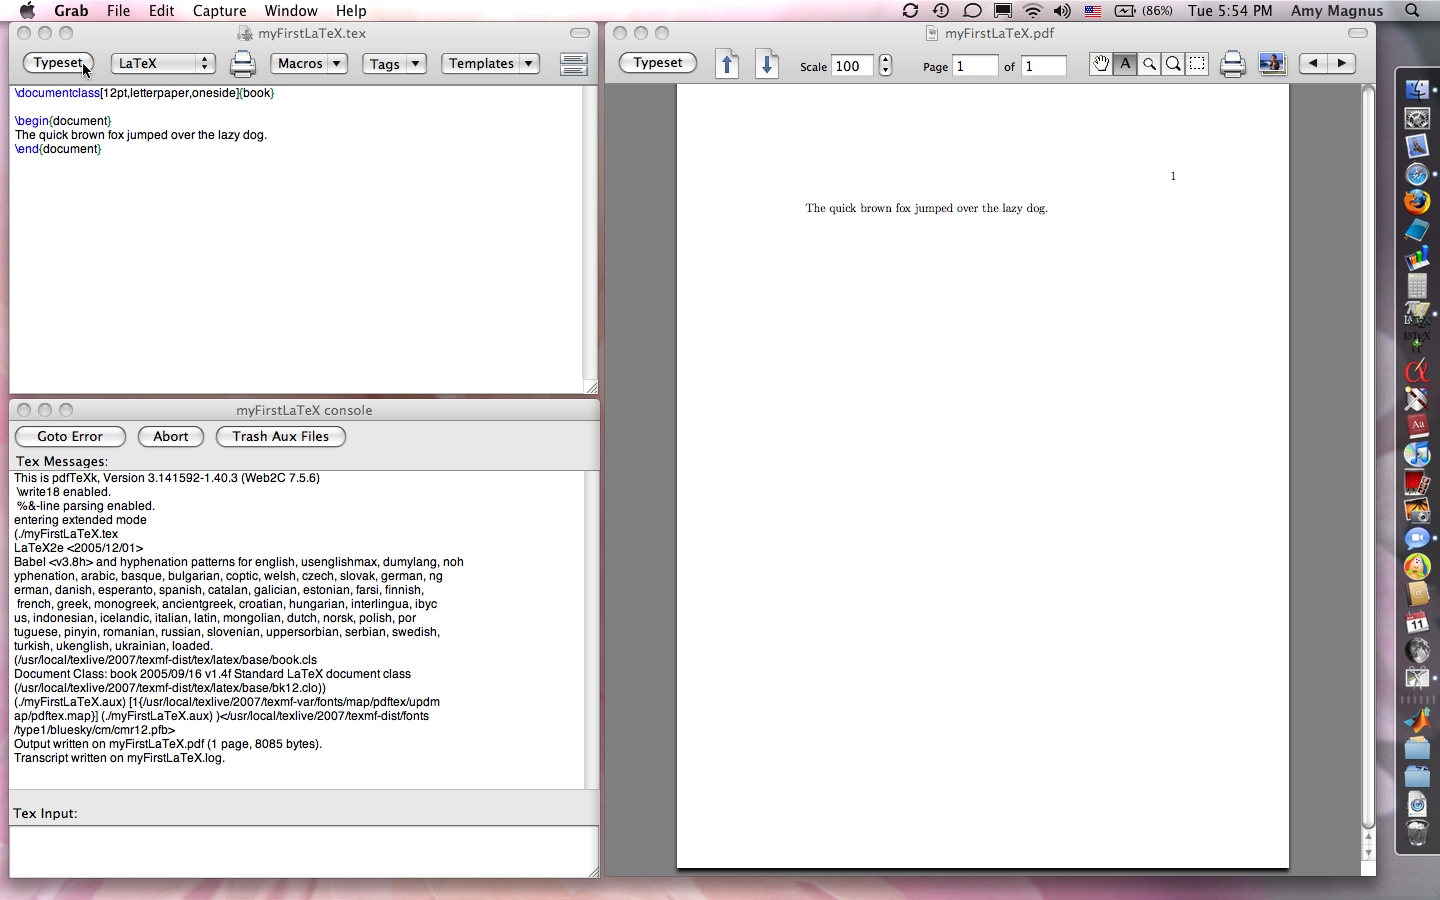
\includegraphics[width=6in]{myFirstLaTeXCursor}
     \caption[\LaTeX\ a very simple document]{Compile a very simple document.}
     \label{fig:MyFirstLaTeX}
 \end{center}
 \vspace{-0.2 in}
\end{figure}
}


\newcommand{\figafitStyle}{\begin{figure}[tbp]
 \begin{center}
    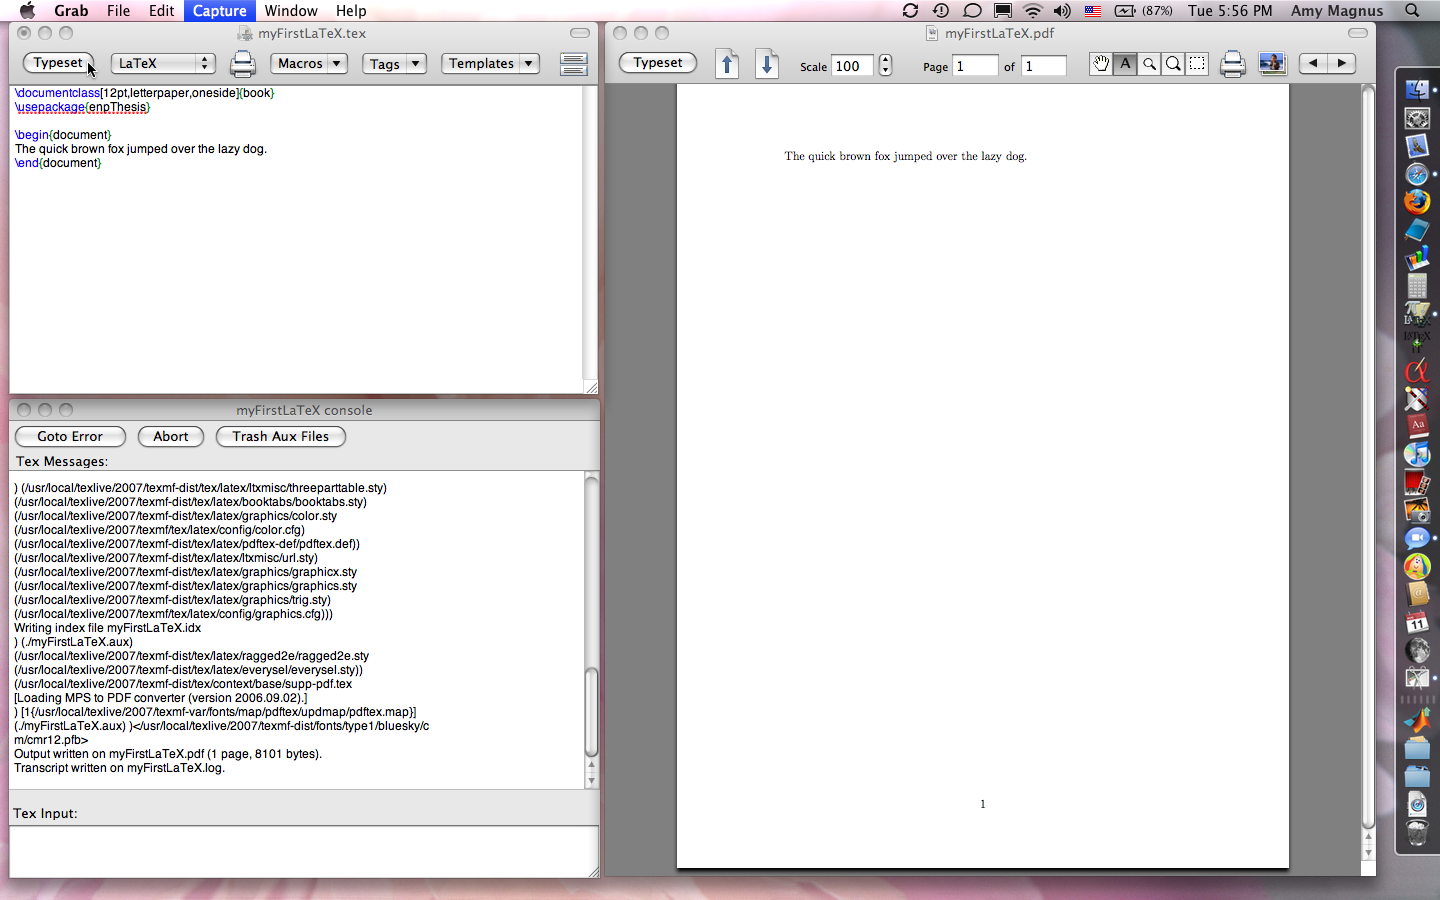
\includegraphics[width=6in]{myFirstLaTeXafit}
     \caption{Recompile using afitThesis.sty, the AFIT
     thesis style file.}
     \label{fig:afitStyle}
 \end{center}
\end{figure}
}


\newcommand{\figtitlePage}{\begin{figure}[tbp]
 \begin{center}
    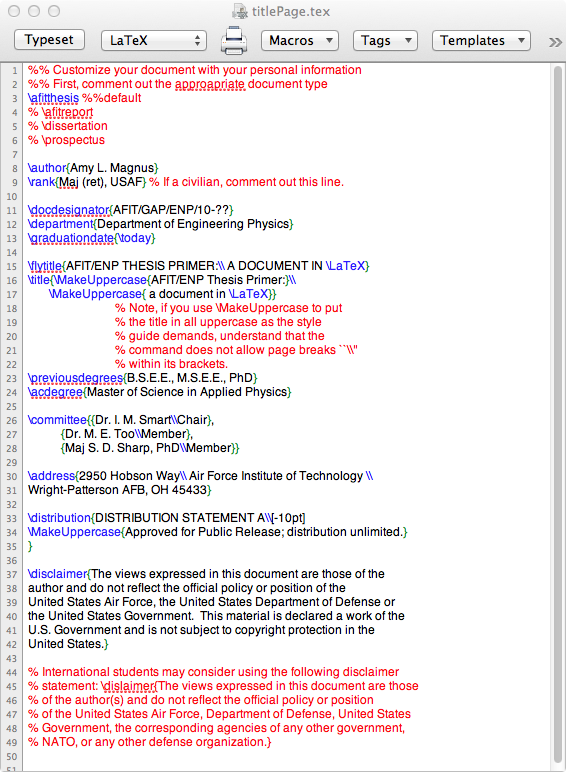
\includegraphics[width=6in]{titlePage}
     \caption{Enter student data in titlePage.tex to customize the
     document's first pages.}
     \label{fig:titlePage}
 \end{center}
\end{figure}
}

\newcommand{\figmyFlypage}{\begin{figure}[tbp]
 \begin{center}
    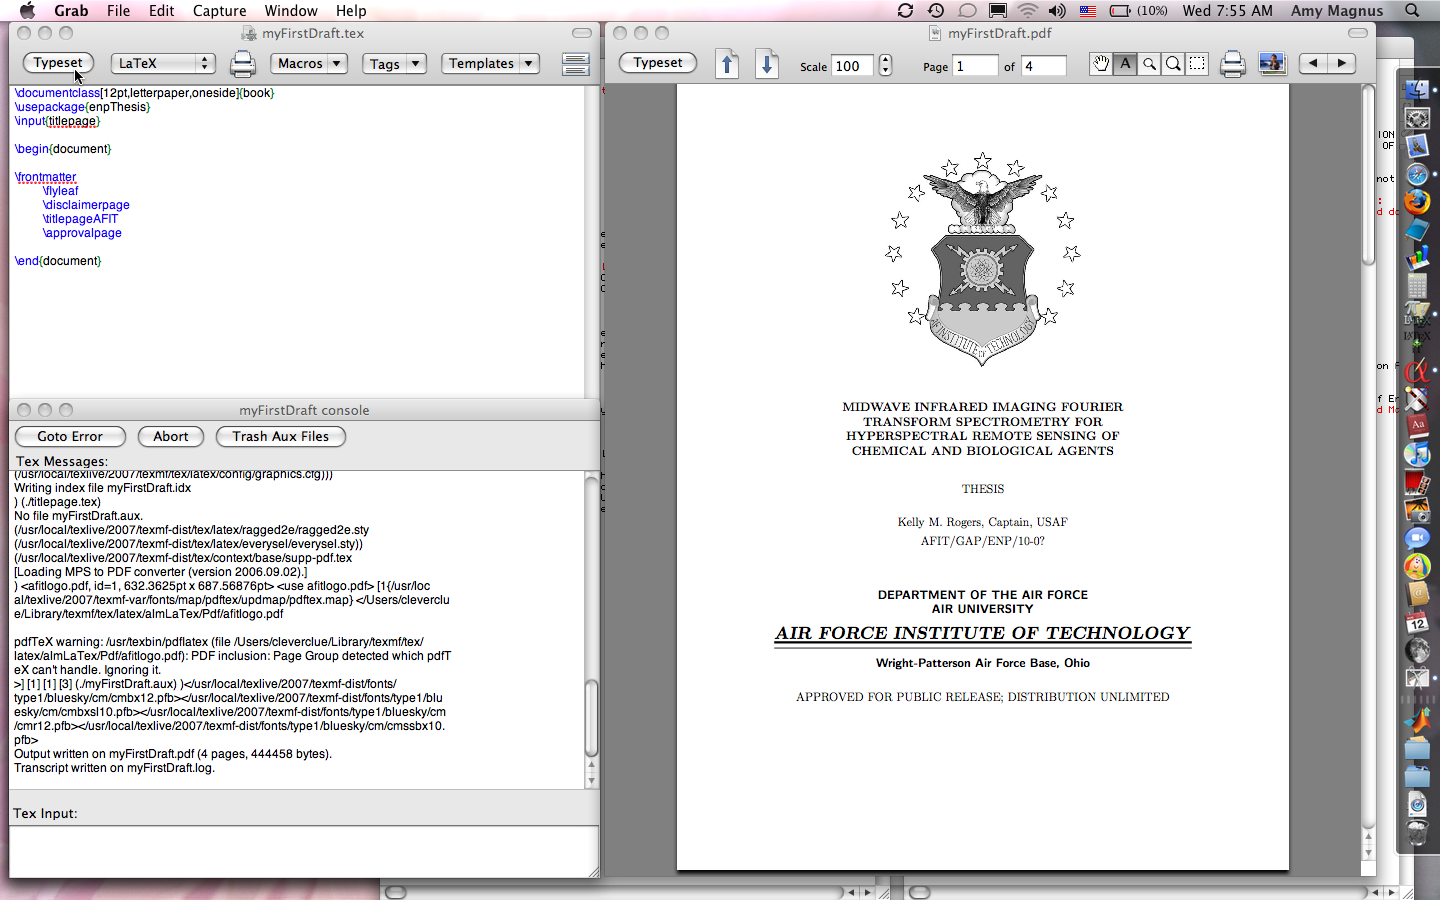
\includegraphics[width=6in]{myFlypage}
     \caption{Here we have compiled the first four page of a thesis.}
     \label{fig:myFlypage}
 \end{center}
\end{figure}
}

\newcommand{\figmyFirstAbstract}{\begin{figure}[tbp]
 \begin{center}
    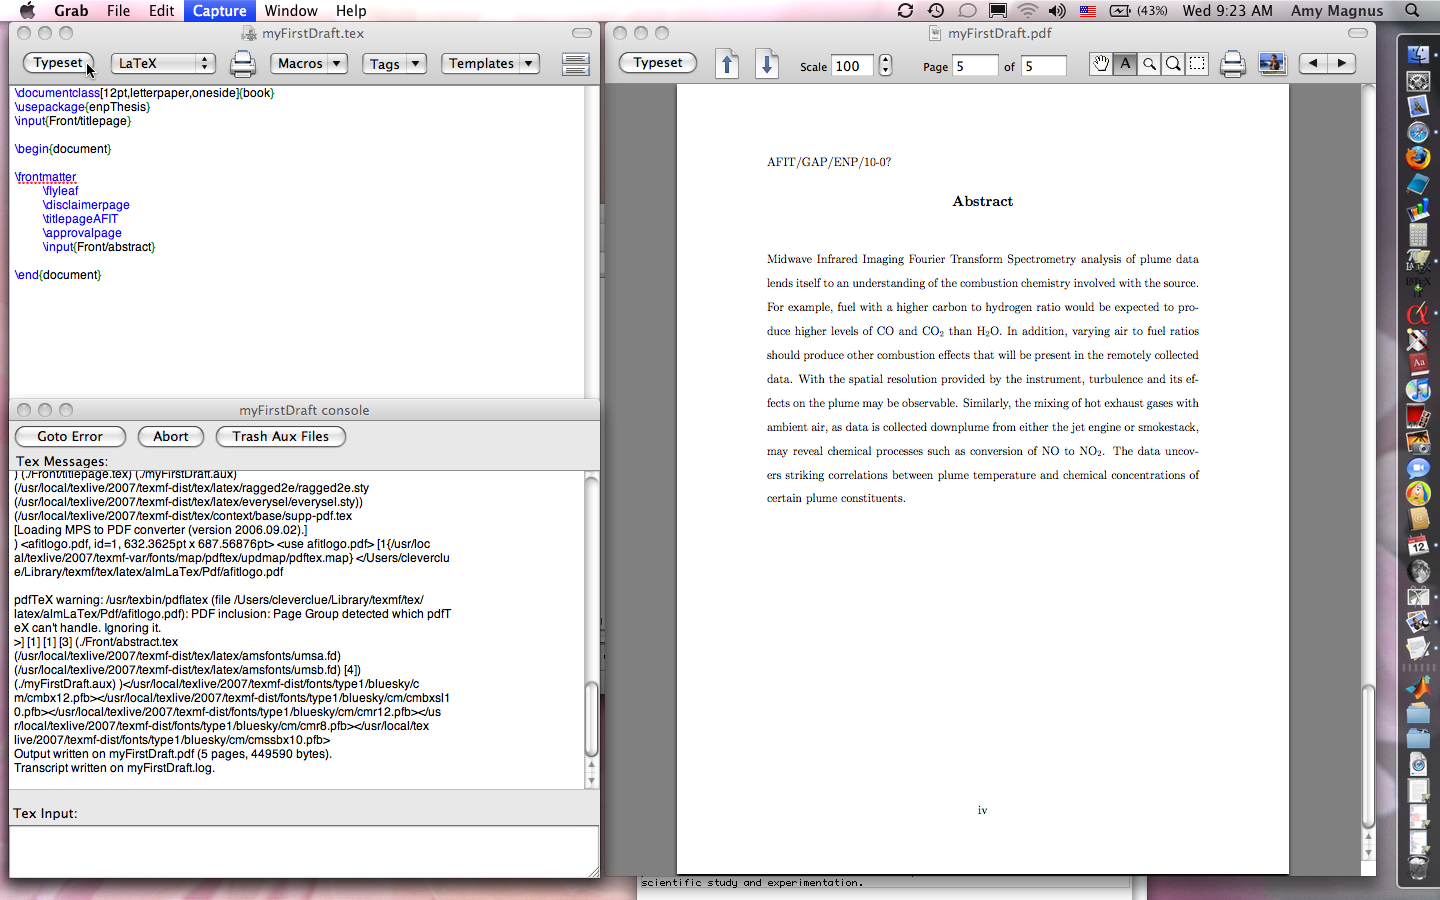
\includegraphics[width=6in]{myFirstAbstract}
     \caption{Add an abstract to the front matter of your thesis.}
     \label{fig:myFirstAbstract}
 \end{center}
\end{figure}
}

\newcommand{\figmyFigures}{\begin{figure}[tbp]
 \begin{center}
    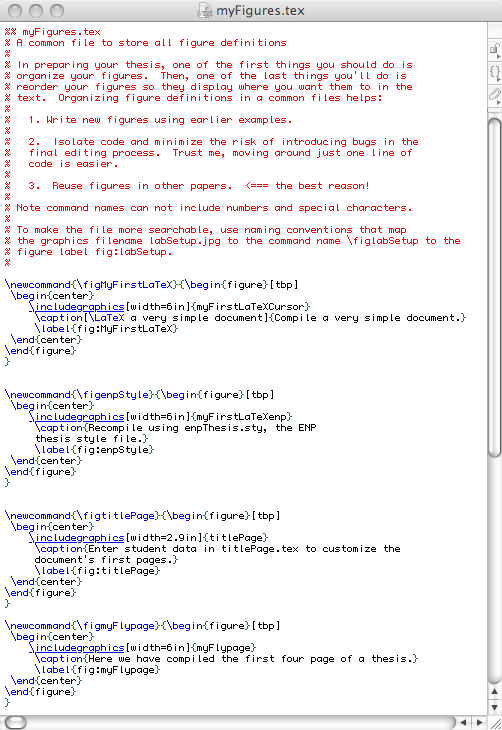
\includegraphics[width=5in]{myFigures}
     \caption{Consider defining all your figures in one file.}
     \label{fig:myFigures}
 \end{center}
\end{figure}
}


\newcommand{\figmyFirstFigures}{\begin{figure}[tbp]
 \begin{center}
    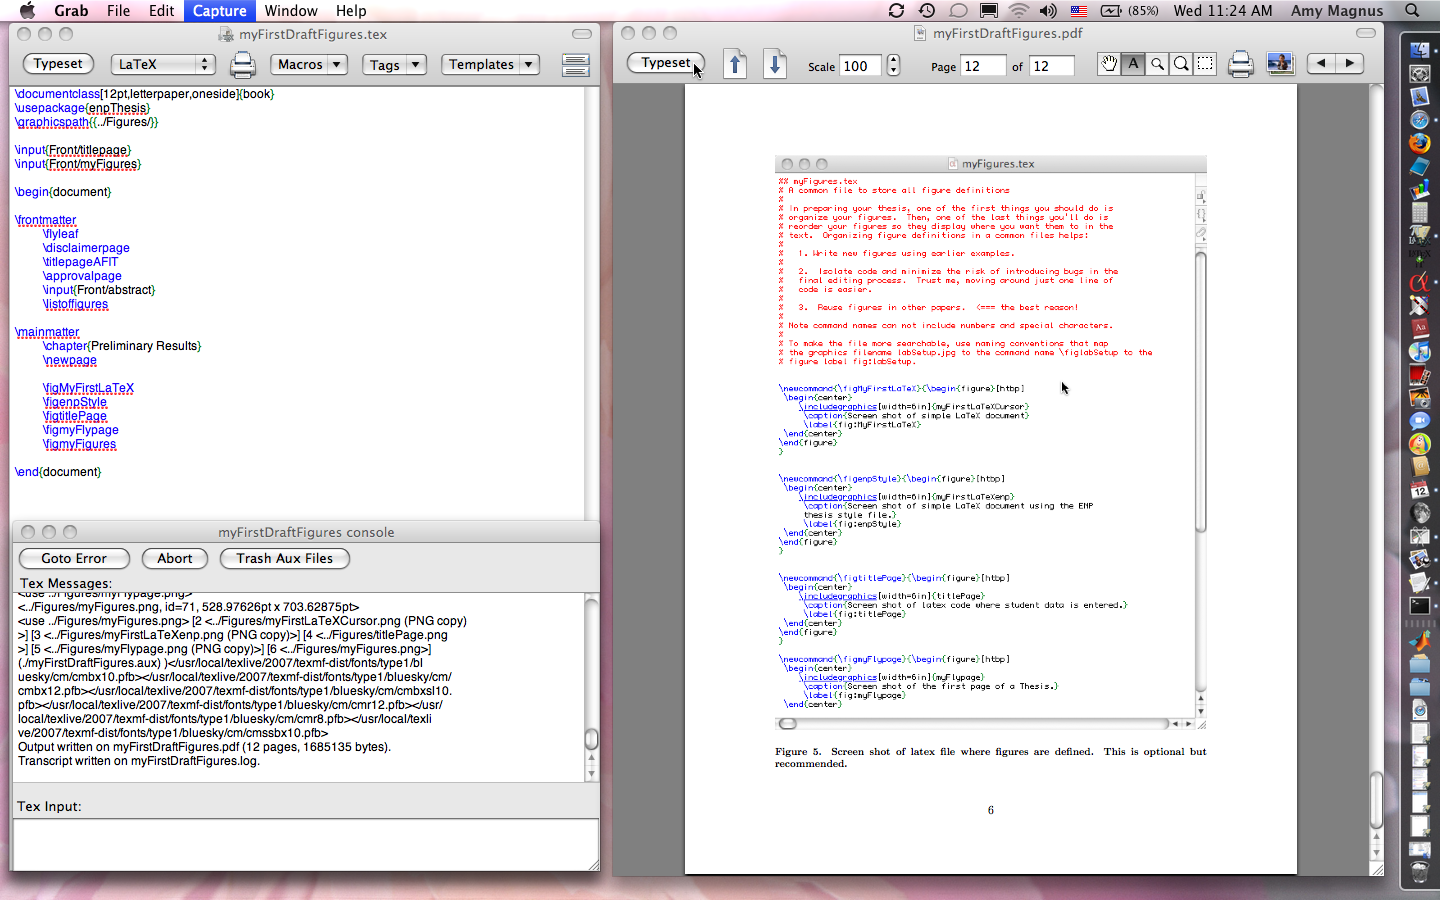
\includegraphics[width=6in]{myFirstFigures}
     \caption{Add figures in the main matter of your document; fill in
     the document around your graphics.}
     \label{fig:myFirstFigures}
 \end{center}
\end{figure}
}

\newcommand{\figmyFirstBibTeX}{\begin{figure}[tbp]
 \begin{center}
    \includegraphics[width=6in]{myFirstBibTeX}
     \caption{Add your bibliography.}
     \label{fig:myFirstBibTeX}
 \end{center}
\end{figure}
}




% define custom commands
\newcommand{\regmark}{\raisebox{5pt}{\tiny \circledR}\xspace}
\newcommand{\matlab}{\textsc{Matlab}\regmark}
\newcommand{\trademark}{\raisebox{5pt}{\tiny TM}\xspace}
\newcommand{\mca}{\texttt{Mathematica}\regmark}
\newcommand{\Latex}{\LaTeX\xspace}

% Create a new theorem style called a Corollary.
% If you don't have any, then just comment this out.
%\theoremstyle{plain} % Default
\newtheorem{cor}{Corollary}[chapter]

%Custom Commands for Student

\newcommand{\primerAddress}{{L:$\backslash$Courses$\backslash$PHYS$\backslash$LaTeX}\xspace}


\begin{document}
\frontmatter
        \flyleaf                        
        \disclaimerpage                 
        \titlepageAFIT                      
        \committeepage  
        % !TEX root = ../SteadmanThesis.tex
\begin{abstract}
Storm enhanced densities (SEDs) are ionospheric plasma enhancements that disrupt radio communications in the near-Earth space environment, degrading the Global Positioning System (GPS) and other high-frequency systems.  Accurate GPS/total electron content (TEC) correction maps produced by ionosphere models can mitigate degradations from SEDs.  An artificial SED was created and ingested via slant TEC measurements into the Global Assimilation of Ionospheric Measurements Gauss-Markov Kalman Filter Model to determine how many ground GPS receivers are needed to produce reliable GPS/TEC correction maps over the continental United States during geomagnetic storming.  It was found that 110 well-positioned GPS receivers produced the best overall TEC accuracy, although significantly improved accuracy was still achieved if 40 or more receivers were used.  It was determined that receiver positioning had a greater impact on TEC accuracy than the number of receivers.  Additionally, it was found that TEC accuracy for the SED region increased at the expense of TEC accuracy everywhere else on the map.
\end{abstract}


        \tableofcontents
        \listoffigures
        

\begin{preface}
Welcome to the world of \Latex! Learn \Latex and you can rapidly
produce papers tailored for a wide variety of publications.
When you create a digital
document\ldots whether you use a ``what you see is what you get''
(WYSIWYG) interface like Microsoft Word or a typesetting system like
\Latex\ldots you are writing a program.  In the realm of academic publishing,
\Latex helps us write a better program.   

The best reasons to write with \Latex are high quality equations,
superior graphics, and the automated generation of table of contents,
lists, and bibliographies.  We can create clean 50+ page documents
that reformat in a snap.  Additionally, due to the fact that the
\Latex typesetting system was written by and for academics, many
of its tools are free and run on Microsoft Windows, Mac OS X, and
Linux.

So let's get started.  Download a \Latex distribution for 
your computer platform, set up your editor and compiler and we'll get 
cracking.  
\end{preface}



\mainmatter
        \chapter{The First Steps}
                Take the first steps in writing your thesis using the simple programs
described in this chapter as a guide.  The source code and support files can be
found on the student drive \primerAddress.  With a
current \Latex distribution\footnote{\Latex distributions update
annually in June.  As of June 2014, the current \Latex
distributions are MiKTeX 2.9 for Windows, TeX Live 2014 for Linux, and
MacTeX 2014 for Macintosh.}, you will be able to compile these programs
without hiccup.

The directory tree below provides a recommended file structure
for the papers generated in your research.  Directories follow ``$>$'' signs; 
standared\ files are
specified in parentheses. 
{\singlespace
\begin{lstlisting}
> myLatexDocuments
  >> afitStyleFiles (afitThesis.sty)
  >> Figures (afitlogo.pdf, afitlogo.eps)
  >> Thesis  (myThesis.tex)
     >>> Preamble (titlePage.tex,myFigures.tex)
     >>> Front (abstract.tex)
     >>> Chapter01 (sectionOne,sectionTwo,...)
     >>> Chapter02 
     . . .
     >>> Appendix01
     . . .
  >> Archived Draft of Thesis 
  >> Archived Perspectus 
  >> Paper One
  >> Paper Two
\end{lstlisting}
} \noindent In a parent directory, create three directories
``afitStyleFiles'', ``Figures'', and ``Thesis''.  Place your graphics
(such as afitlogo.pdf) in the directory Figures, your \Latex style
files (afitThesis.sty, sf298.sty, sf298.dtx, and sf298.ins) in
afitStyleFiles, and the latex code for your thesis document in Thesis.
Organized in this way, the files in the Figures directory and the
afitStyleFiles directory can be used by your thesis, perspectus, archived drafts,
and other publications.  Typically, graphics account for most of the
memory taken up by a digital document, and this efficiency in
sharing saves significant disk space.



		
                \figMyFirstLaTeX
                \section{\Latex a simple document}
                To compile a LaTex document, start simple with the code listed 
below.  Store the code as a .tex file in your
Thesis directory. Then compile the code to test the set up of your \Latex 
distribution and compiler\footnote{Popular compilers include TeXworks 
and TeXShop.}.  Figure~\ref{fig:MyFirstLaTeX} provides a screen
shot of the typeset document with its compilation aids.

 {\singlespace   
 \begin{verbatim}
\documentclass[12pt,letterpaper,oneside]{book}
 
\begin{document}
The quick brown fox jumped over the lazy dog.
\end{document}
\end{verbatim}
} 
\noindent The code has two parts: the preamble and the body.  The
preamble establishes the default formatting for the document; the body
holds the content.  The preamble starts with a {\bf $\backslash$documentclass}
declaration and ends at the {\bf $\backslash$begin\{document\}}
command. The {body} is placed in between the {\bf
$\backslash$begin\{document\}} and {\bf $\backslash$end\{document\}}
commands. 

In the preamble of this first document, Here we have selected a one
sided, 12-pt font book format.  In the body, let us enter a short
phrase---just to get a feel for how content is added---that includes 
all characters in the Roman alphabet.
    
   
%Other formats include article, report, memoir The body contains the
%actual content.


		

                \figafitStyle
                \section{Add a style file}
                Next, we add the style file afitThesis.sty to the preamble and
recompile.  The style file implements the AFIT thesis format and is
added via the command {\bf $\backslash$usepackage}.

\vspace{-0.3in}
{\singlespace
\begin{verbatim}
\documentclass[12pt,letterpaper,oneside]{book}
\usepackage{../afitStyleFiles/afitThesis}

\begin{document}
The quick brown fox jumped over the lazy dog.
\end{document}
\end{verbatim}
} \noindent Note the resulting changes to the document in
Figure~\ref{fig:afitStyle}.  Some adjustments are immediately apparent:
The margins have changed and a page number is now located at the
bottom of the page.
    

		

                \figtitlePage
                \section{Add the front matter}
                The style file {\em afitThesis.sty} contains code that generates the
first, standardized pages of the thesis document.  Theses pages are the
flyleaf, disclaimer page, the title page, and the committee page.  For
each thesis, we customize these four pages by editing a tex file
called {\em titlePage.tex}.  The customizable items for a thesis are:

\vspace{-0.15in}
\begin{tabular}{p{2.2in}p{4in}}
    \begin{itemize}\itemsep-10pt
	    \item Author
	    \item Rank
	    \item Graduation Date
	    \item Document Designator
	    \item Flypage title
	    \item Title
     \end{itemize} &
    \begin{itemize}\itemsep-10pt
	    \item Previous degrees
	    \item Academic degree upon AFIT graduation
	    \item Committee membership
	    \item Department granting your degree
	    \item School address
	    \item Distribution statement
	    \item Disclaimer
     \end{itemize} 
\end{tabular}

\noindent Add this information to {\em titlePage.tex} as you obtain
it.  One item to include as soon as possible is the distribution
statement; ask your advisor which distribution statement is
appropriate for your draft document.
    
If your document is something other than a thesis, you can set a flag at
the beginning of {\em titlePage.tex}.  Use the $\%$ symbol to comment
out unused flags and remove the $\%$ from the line of the
appropriate flag.  In this way, the correct flag will execute at
compilation.  The available flags correspond to the following
documents:

\vspace{-0.3in}
{\singlespace
\begin{center}
\begin{tabular}{|l|l|}
    \hline
    \bf Document & \bf Flag\\
    \hline
    Thesis & {\bf $\backslash$afitthesis}  \\
    Report & {\bf $\backslash$afitreport} \\
    Dissertation & {\bf $\backslash$dissertation} \\
    Prospectus & {\bf $\backslash$prospectus}\\
    \hline
\end{tabular}
\end{center}}

Once you customize the {\em titlePage.tex} file, we can typeset
the first four pages of an AFIT thesis: the flypage, the disclaimer
page, the title page and the committee page. 

We must add a few lines to our typesetting program.  Within the
document environment, we list the first four pages (See line 7-11)
under front matter.  The flypage includes our first graphic---the AFIT
logo---so we provide a path to our figures by using the {\bf
$\backslash$graphicspath} command\footnote{Note the double brackets
used in the graphicspath command; they are necessary for the command
to execute properly with some compilers.} in the preamble.  Note line
3 below where we set the path.  The {\em titlePage.tex} provides
customization, not content, so it is called in the preamble;
call the file by using the command {\bf $\backslash$input} as in line
4 of the code below.  In all, we have added seven lines of code to our
short program to create a four page document.

\vspace{-0.25in}
{\singlespace
\begin{verbatim}
\documentclass[12pt,letterpaper,oneside]{book}
\usepackage{afitThesis}
\graphicspath{{..\Figures}}
\input{Preamble/titlepage}

\begin{document}
\frontmatter
        \flyleaf                        
        \disclaimerpage                 
        \titlepageAFIT                      
        \committeepage  	
\end{document}
\end{verbatim}
}


                \figmyFlypage
                
\noindent The next section to add to the front matter is an abstract.
Create a file {\em abstract.tex} and place the text for the abstract
between the commands {\bf $\backslash$begin\{abstract\}} and {\bf
$\backslash$end\{abstract\}} as below.

\vspace{-0.3in}
{\singlespace
\begin{verbatim}
\begin{abstract}
    Midwave Infrared Imaging Fourier Transform Spectrometry analysis of
    plume data lends itself to an understanding of the combustion
    chemistry involved with the source. ...
\end{abstract}
\end{verbatim}
}

Above, we use a construct called an environment.  There are several
enviroments: figure, itemize,
verbatim, quote, equation to name a few.  \Latex friendly editors will
help you build these environments.  The abstract environment is
actually a customized environment created in the {\em afitThesis.sty}
file; thus, it will not be found in the common \Latex literature or
tools; but, as you can see above, it is simple to implement.



                \figmyFirstAbstract
                Other common items that can be added to the front matter are
acknowledgements, the table of contents and lists of figures and
tables.  The acknowledgements can be added in the same manner as the
abstract; use the environment commands for the
Acknowledgement: {\bf $\backslash$begin\{acknowledgement\}} and {\bf
$\backslash$end\{acknowledgement\}}.  The table of contents and other lists
build automatically as you add sections, figures, and tables and are placed
in the front matter using the commands below.  

\vspace{-0.3in} {\singlespace
\begin{verbatim}
\frontmatter
        \flyleaf                        
        \disclaimerpage                 
        \titlepageAFIT                      
        \committeepage
        % !TEX root = ../SteadmanThesis.tex
\begin{abstract}
Storm enhanced densities (SEDs) are ionospheric plasma enhancements that disrupt radio communications in the near-Earth space environment, degrading the Global Positioning System (GPS) and other high-frequency systems.  Accurate GPS/total electron content (TEC) correction maps produced by ionosphere models can mitigate degradations from SEDs.  An artificial SED was created and ingested via slant TEC measurements into the Global Assimilation of Ionospheric Measurements Gauss-Markov Kalman Filter Model to determine how many ground GPS receivers are needed to produce reliable GPS/TEC correction maps over the continental United States during geomagnetic storming.  It was found that 110 well-positioned GPS receivers produced the best overall TEC accuracy, although significantly improved accuracy was still achieved if 40 or more receivers were used.  It was determined that receiver positioning had a greater impact on TEC accuracy than the number of receivers.  Additionally, it was found that TEC accuracy for the SED region increased at the expense of TEC accuracy everywhere else on the map.
\end{abstract}


        \input{Front/acknowledgement}
        \tableofcontents
        \listoffigures
        \listoftables
\end{verbatim}
}

\noindent The order follows the AFIT style guide\cite{AFITStyle}.  The {\em
afitThesis.sty} defines additional environments and lists.  We
will describe how to implement those items in the next chapter.
For now, we will simply keep the abstract and perhaps the list of
figures in our front matter as we move on to the
main body of the thesis.






                \section{Add figures to the main matter and start writing}
                \figmyFigures
                
To concentrate on your research, consider organizing your figures
first.  Build the document around your figures, and you will be able
to concentrate on the story of your contribution---not the work that
has gone on before.  

To organizing your figures, it is helpful to define them in a
common file.  See {\em myFigures.tex} depicted in
Figure~\ref{fig:myFigures} and stored in the Preamble subdirectory.
In this way, you may:
    \begin{itemize}
      \item Readily write new figures using earlier examples. 
      
      \item  Isolate code and minimize the risk of introducing bugs in the
      final editing process.  Moving around one line of
      code is easy and safe.
      
      \item Standardize figures without having to locate them 
      throughout the document.
      
      \item  Reuse figures in other papers.  $\leftarrow$ The best reason!
    \end{itemize}
        
\noindent In {\em myFigures.tex}, use {\bf
$\backslash${newcommand}} to define a command for each figure as
below:

{\vspace{-.30in}}
{\singlespace
\begin{verbatim}
\newcommand{\figmyFigures}{
    \begin{figure}[htbp]
        \begin{center}
             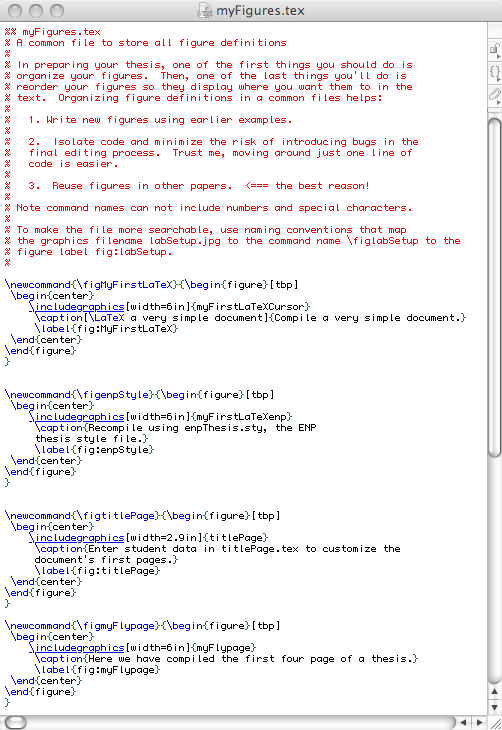
\includegraphics[width=6in]{myFigures}
             \caption{A sample tex file where figures are defined.}
             \label{fig:myFigures}
        \end{center}
    \end{figure}
}
\end{verbatim}}
    
\noindent For a command, chose a naming convention that
intuitively links the command to the graphic file and the figure
label.  For example, above we have defined a command {\bf
$\backslash${figmyFigures}} to position a figure containing graphic
myFigures.png.  Note command names cannot include numbers or special
characters.



                \figmyFirstFigures
                
Now, in the preamble of your code, input {\em myFigures.tex} in the
same manner as you input {\em titlepage.tex}.  Now we are ready to add
the main body of the thesis.  Initiate the main body of your document
by calling the {\bf$\backslash$mainmatter} command.  Next, call the
figures that you have defined and compile.  Note, once you add a
chapter, you can remove {\bf$\backslash$thispagestyle\{plain\}} which
precedes the {\bf$\backslash$mainmatter} command.

\vspace{-0.3in}
{\singlespace
\begin{verbatim}
\documentclass[12pt,letterpaper,oneside]{book}
\usepackage{afitThesis}
\graphicspath{{..\Figures}}
\input{Preamble/titlepage}
%% myFigures.tex
% A common file to store all figure definitions
%
% In preparing your thesis, one of the first things you should do is
% organize your figures.  Then, one of the last things you'll do is
% reorder your figures so they display where you want them to in the
% text.  Organizing figure definitions in a common files helps:
%
%   1. Write new figures using earlier examples.
%
%   2.  Isolate code and minimize the risk of introducing bugs in the
%   final editing process.  Trust me, moving around just one line of
%   code is easier.
%
%   3.  Reuse figures in other papers.  <=== the best reason!
%
% Note command names can not include numbers and special characters.
%
% To make the file more searchable, use naming conventions that map
% the graphics filename labSetup.jpg to the command name \figlabSetup to the
% figure label fig:labSetup.
% 

\newcommand{\figMyFirstLaTeX}{\begin{figure}[tbp]
 \begin{center}
    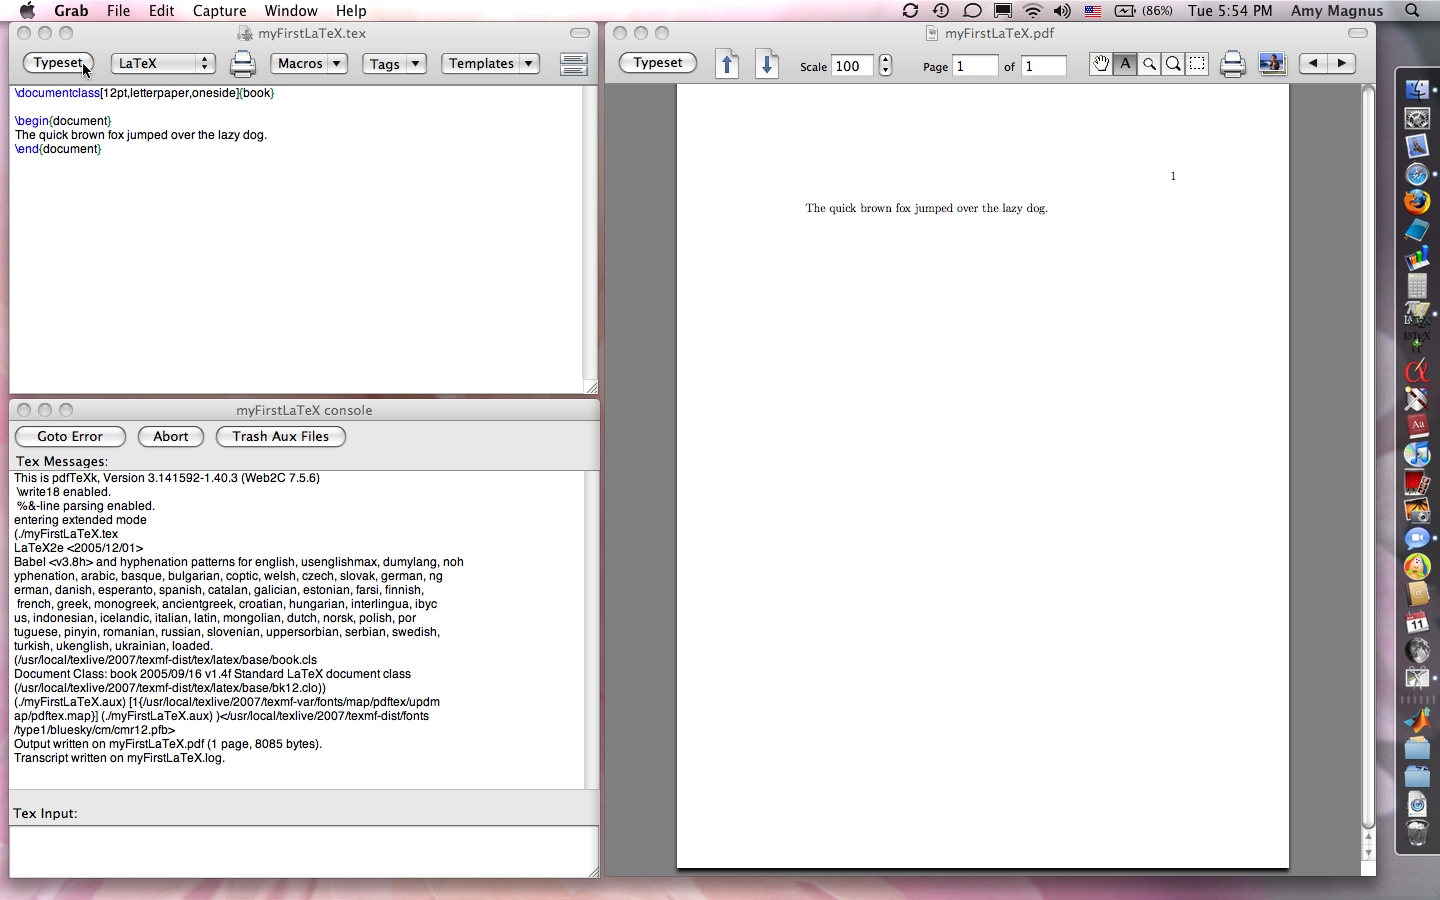
\includegraphics[width=6in]{myFirstLaTeXCursor}
     \caption[\LaTeX\ a very simple document]{Compile a very simple document.}
     \label{fig:MyFirstLaTeX}
 \end{center}
 \vspace{-0.2 in}
\end{figure}
}


\newcommand{\figafitStyle}{\begin{figure}[tbp]
 \begin{center}
    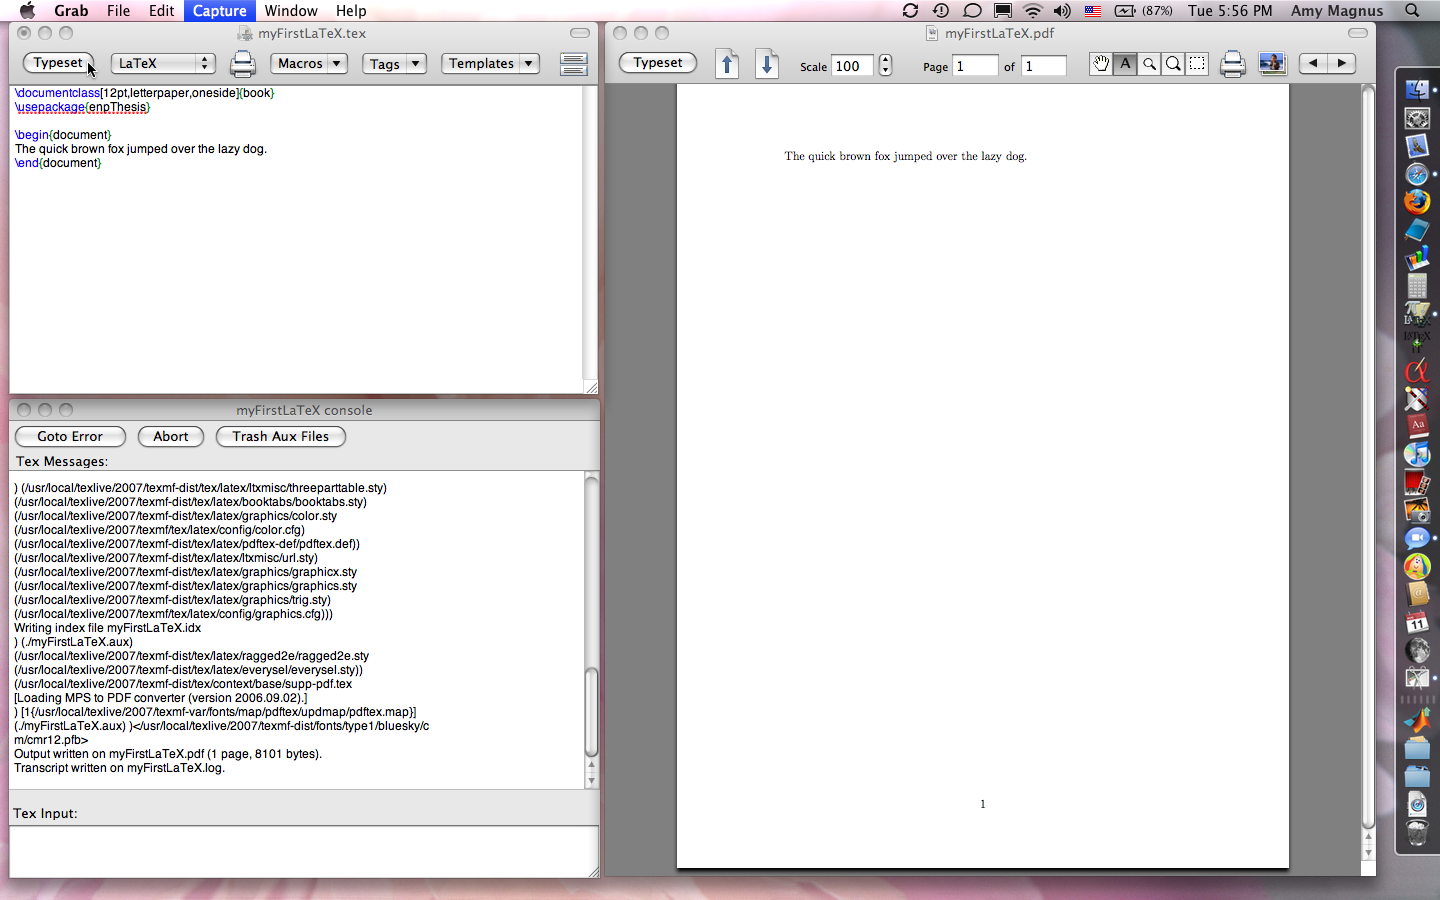
\includegraphics[width=6in]{myFirstLaTeXafit}
     \caption{Recompile using afitThesis.sty, the AFIT
     thesis style file.}
     \label{fig:afitStyle}
 \end{center}
\end{figure}
}


\newcommand{\figtitlePage}{\begin{figure}[tbp]
 \begin{center}
    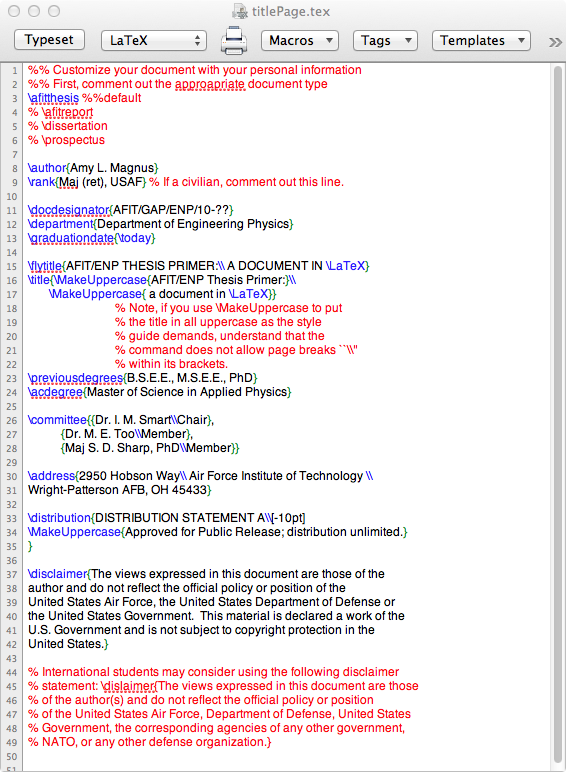
\includegraphics[width=6in]{titlePage}
     \caption{Enter student data in titlePage.tex to customize the
     document's first pages.}
     \label{fig:titlePage}
 \end{center}
\end{figure}
}

\newcommand{\figmyFlypage}{\begin{figure}[tbp]
 \begin{center}
    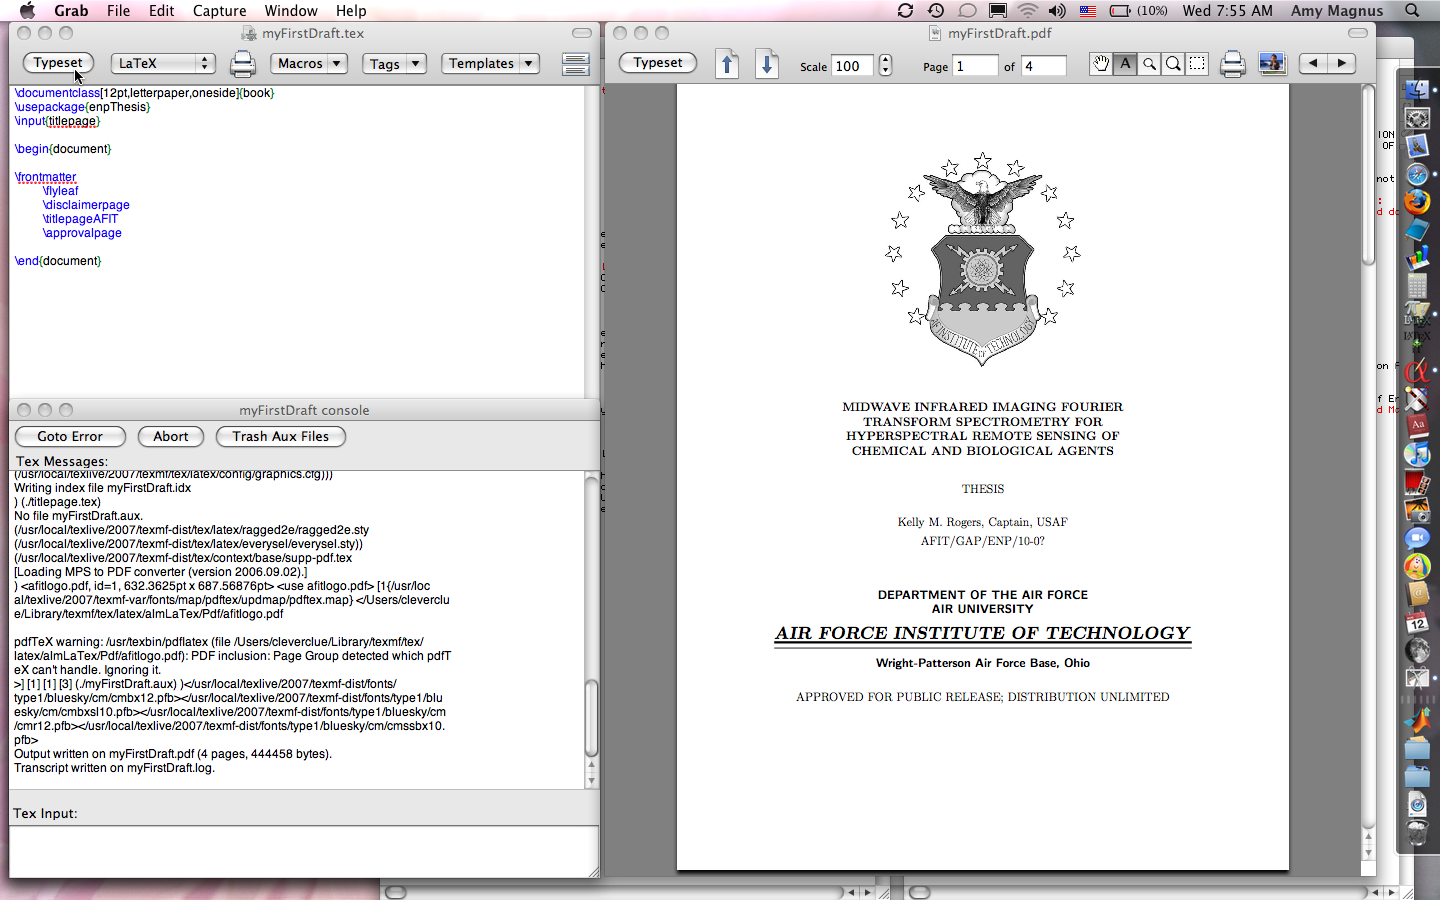
\includegraphics[width=6in]{myFlypage}
     \caption{Here we have compiled the first four page of a thesis.}
     \label{fig:myFlypage}
 \end{center}
\end{figure}
}

\newcommand{\figmyFirstAbstract}{\begin{figure}[tbp]
 \begin{center}
    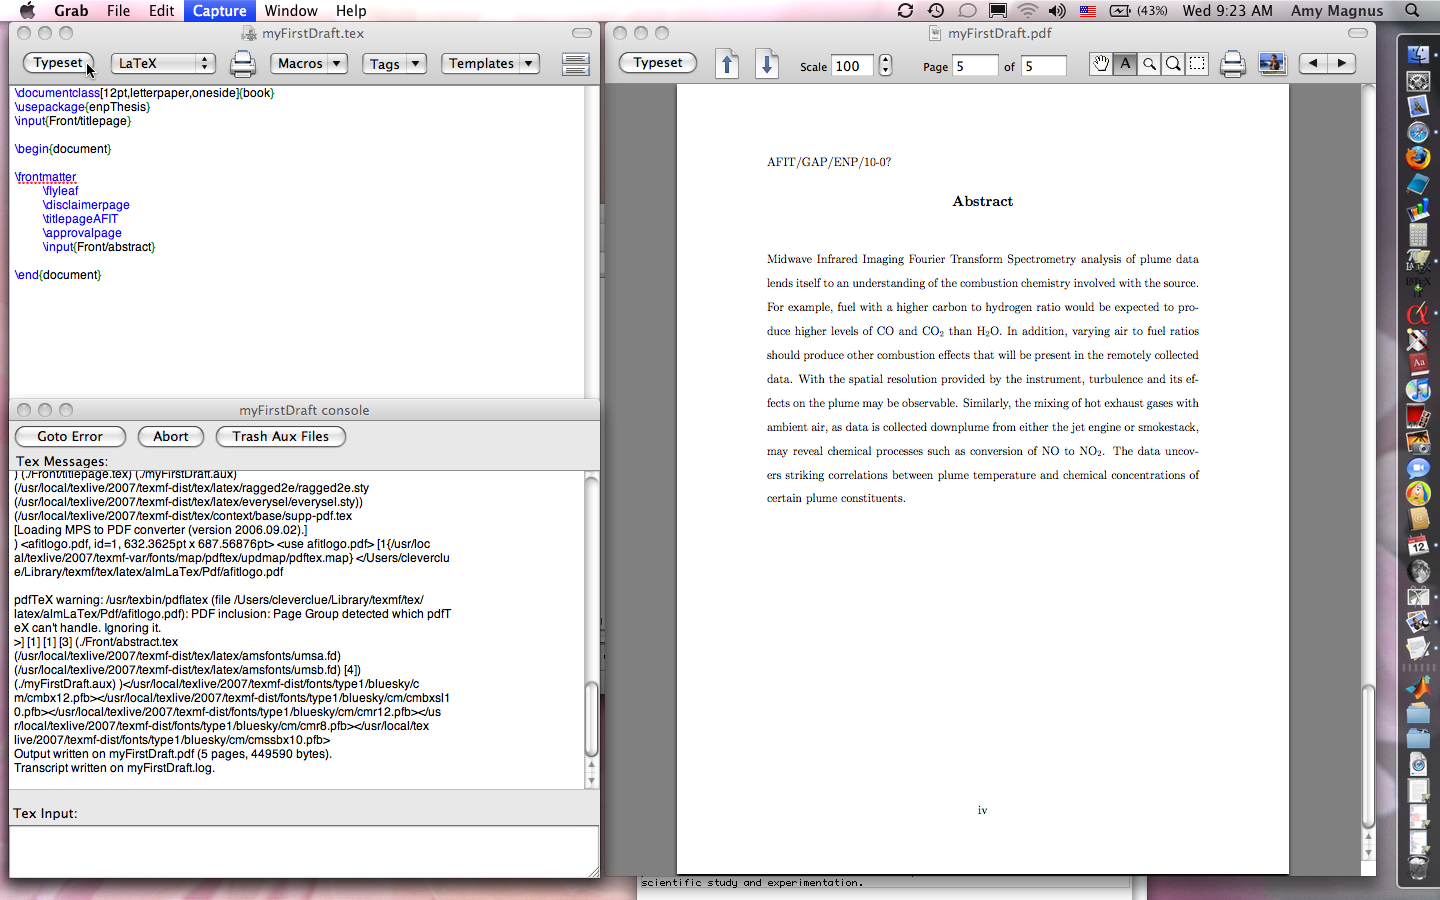
\includegraphics[width=6in]{myFirstAbstract}
     \caption{Add an abstract to the front matter of your thesis.}
     \label{fig:myFirstAbstract}
 \end{center}
\end{figure}
}

\newcommand{\figmyFigures}{\begin{figure}[tbp]
 \begin{center}
    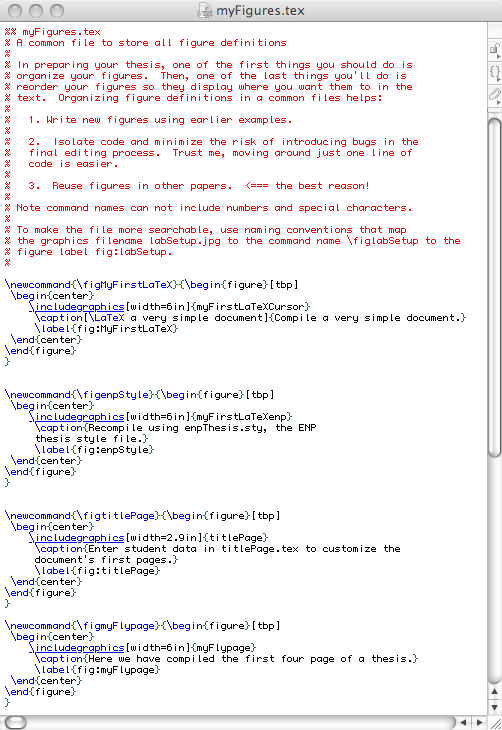
\includegraphics[width=5in]{myFigures}
     \caption{Consider defining all your figures in one file.}
     \label{fig:myFigures}
 \end{center}
\end{figure}
}


\newcommand{\figmyFirstFigures}{\begin{figure}[tbp]
 \begin{center}
    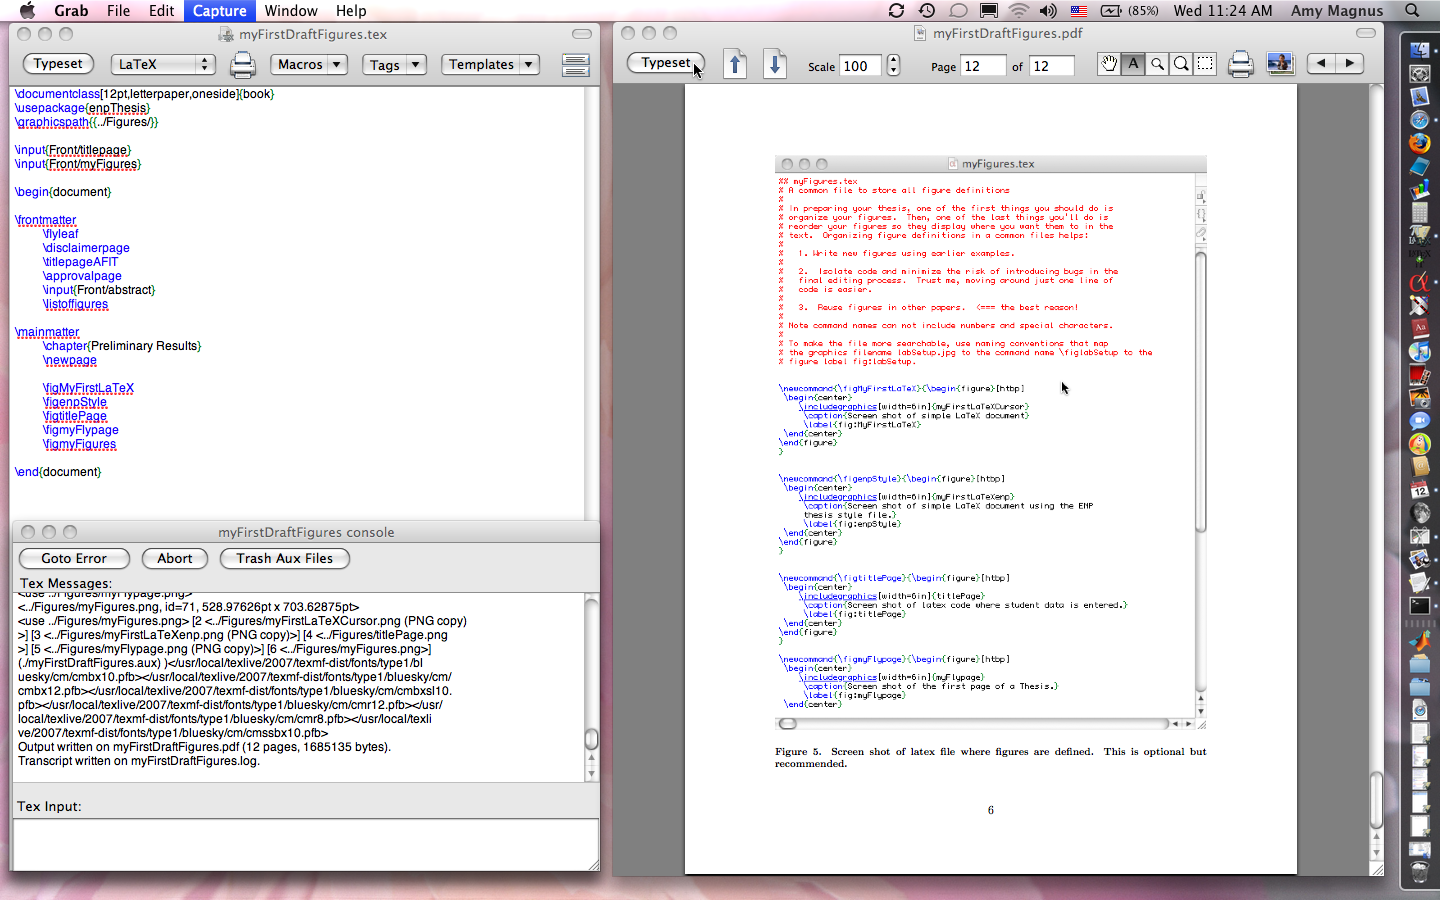
\includegraphics[width=6in]{myFirstFigures}
     \caption{Add figures in the main matter of your document; fill in
     the document around your graphics.}
     \label{fig:myFirstFigures}
 \end{center}
\end{figure}
}

\newcommand{\figmyFirstBibTeX}{\begin{figure}[tbp]
 \begin{center}
    \includegraphics[width=6in]{myFirstBibTeX}
     \caption{Add your bibliography.}
     \label{fig:myFirstBibTeX}
 \end{center}
\end{figure}
}





\begin{document}
\frontmatter
        \flyleaf                        
        \disclaimerpage                 
        \titlepageAFIT                      
        \committeepage  	
        % !TEX root = ../SteadmanThesis.tex
\begin{abstract}
Storm enhanced densities (SEDs) are ionospheric plasma enhancements that disrupt radio communications in the near-Earth space environment, degrading the Global Positioning System (GPS) and other high-frequency systems.  Accurate GPS/total electron content (TEC) correction maps produced by ionosphere models can mitigate degradations from SEDs.  An artificial SED was created and ingested via slant TEC measurements into the Global Assimilation of Ionospheric Measurements Gauss-Markov Kalman Filter Model to determine how many ground GPS receivers are needed to produce reliable GPS/TEC correction maps over the continental United States during geomagnetic storming.  It was found that 110 well-positioned GPS receivers produced the best overall TEC accuracy, although significantly improved accuracy was still achieved if 40 or more receivers were used.  It was determined that receiver positioning had a greater impact on TEC accuracy than the number of receivers.  Additionally, it was found that TEC accuracy for the SED region increased at the expense of TEC accuracy everywhere else on the map.
\end{abstract}


        \tableofcontents
        \listoffigures
\mainmatter
        \figMyFirstLaTeX
        \figafitStyle
        \figtitlePage
        \figmyFlypage
        \figmyFirstAbstract
        \figmyFigures
        \figmyFirstFigures
\end{document}
\end{verbatim}
}
\vspace{-0.1in}

From here, add text around your figures.  To produce this document, we
used the following code:

\vspace{-0.25in}
{\singlespace
\begin{verbatim}
\documentclass[12pt,letterpaper,oneside]{book}
\usepackage{afitThesis}
\graphicspath{{../Figures/}}

\input{Preamble/titlepage}
%% myFigures.tex
% A common file to store all figure definitions
%
% In preparing your thesis, one of the first things you should do is
% organize your figures.  Then, one of the last things you'll do is
% reorder your figures so they display where you want them to in the
% text.  Organizing figure definitions in a common files helps:
%
%   1. Write new figures using earlier examples.
%
%   2.  Isolate code and minimize the risk of introducing bugs in the
%   final editing process.  Trust me, moving around just one line of
%   code is easier.
%
%   3.  Reuse figures in other papers.  <=== the best reason!
%
% Note command names can not include numbers and special characters.
%
% To make the file more searchable, use naming conventions that map
% the graphics filename labSetup.jpg to the command name \figlabSetup to the
% figure label fig:labSetup.
% 

\newcommand{\figMyFirstLaTeX}{\begin{figure}[tbp]
 \begin{center}
    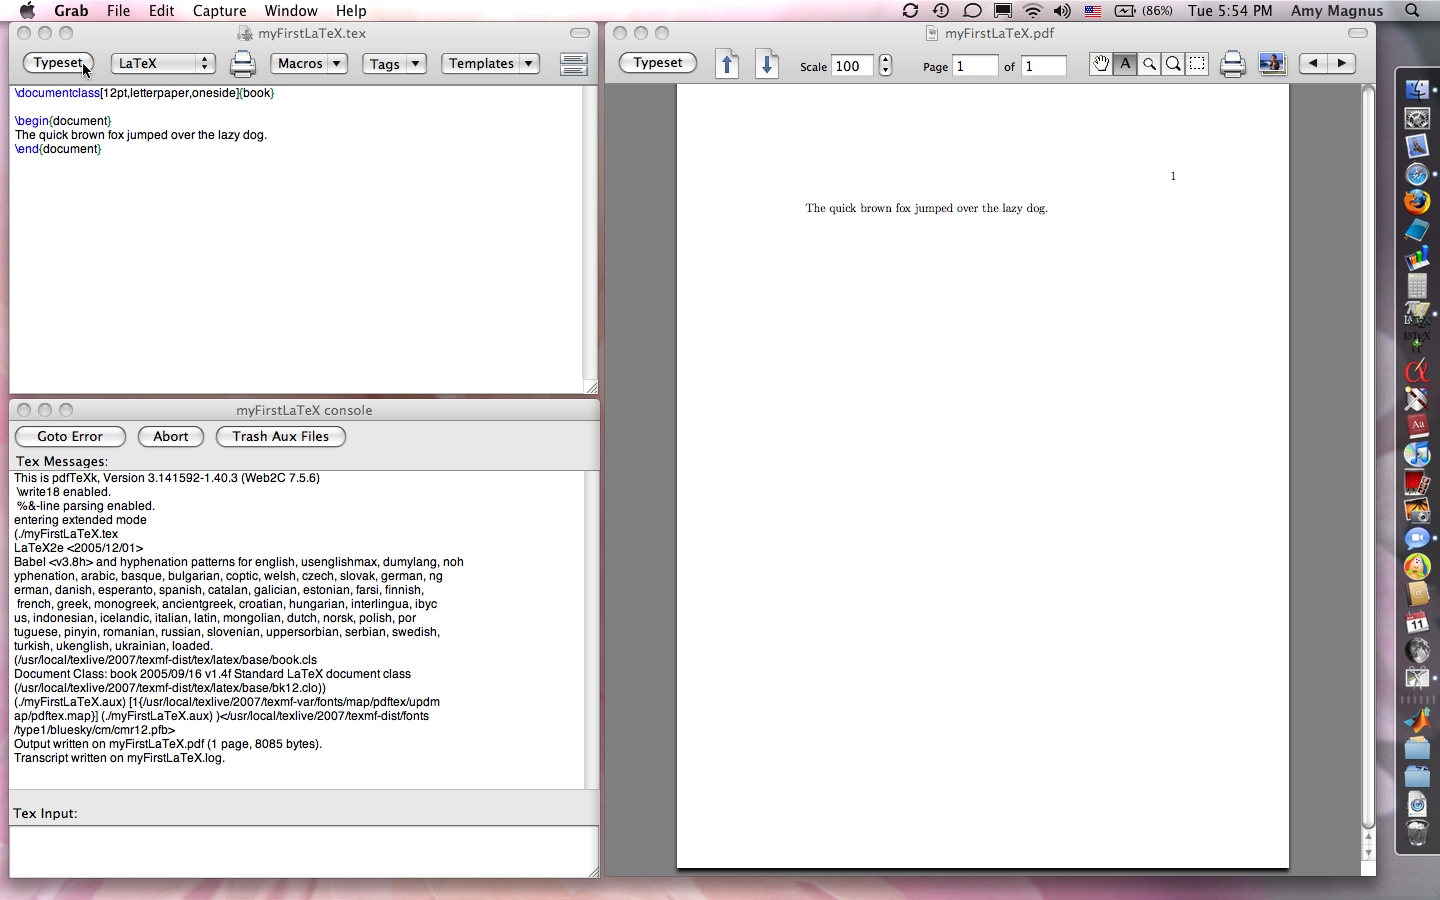
\includegraphics[width=6in]{myFirstLaTeXCursor}
     \caption[\LaTeX\ a very simple document]{Compile a very simple document.}
     \label{fig:MyFirstLaTeX}
 \end{center}
 \vspace{-0.2 in}
\end{figure}
}


\newcommand{\figafitStyle}{\begin{figure}[tbp]
 \begin{center}
    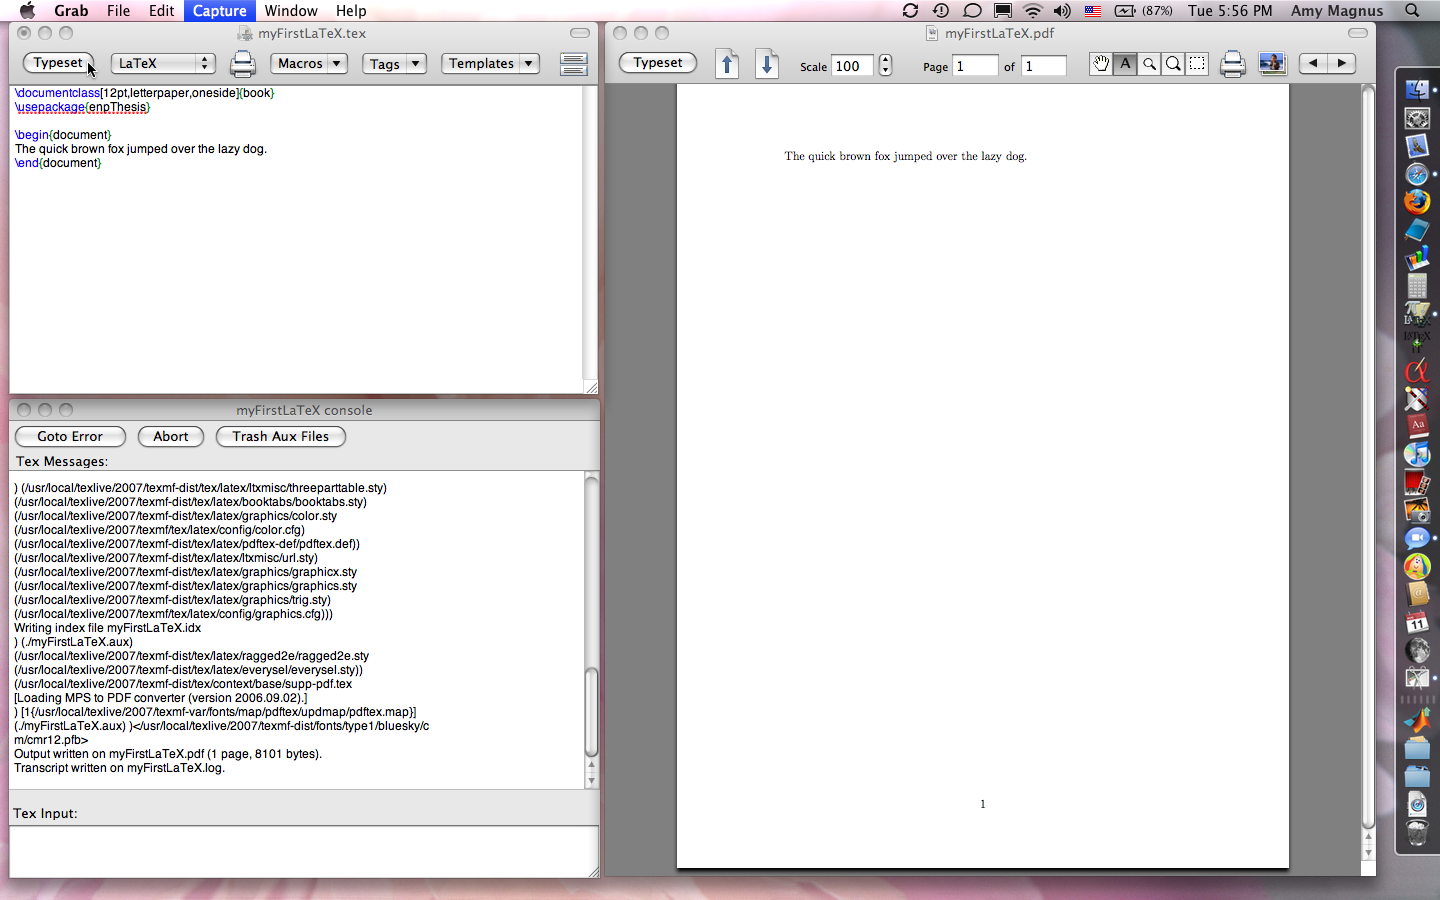
\includegraphics[width=6in]{myFirstLaTeXafit}
     \caption{Recompile using afitThesis.sty, the AFIT
     thesis style file.}
     \label{fig:afitStyle}
 \end{center}
\end{figure}
}


\newcommand{\figtitlePage}{\begin{figure}[tbp]
 \begin{center}
    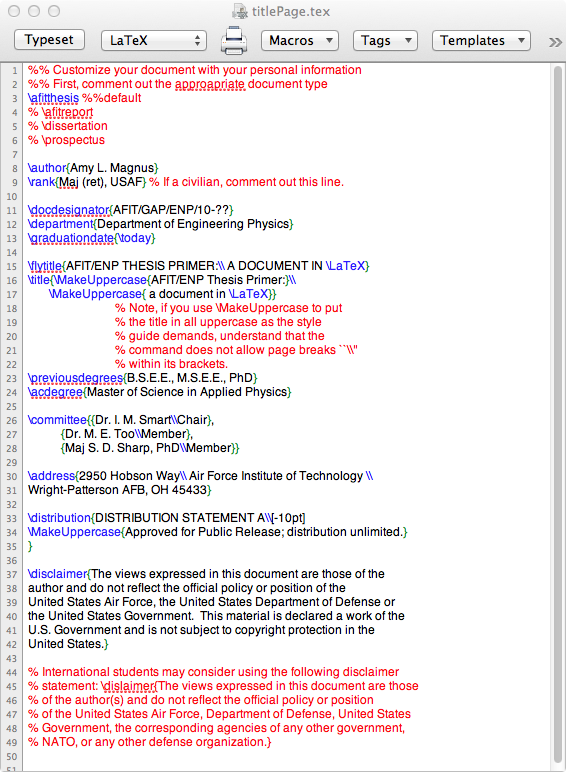
\includegraphics[width=6in]{titlePage}
     \caption{Enter student data in titlePage.tex to customize the
     document's first pages.}
     \label{fig:titlePage}
 \end{center}
\end{figure}
}

\newcommand{\figmyFlypage}{\begin{figure}[tbp]
 \begin{center}
    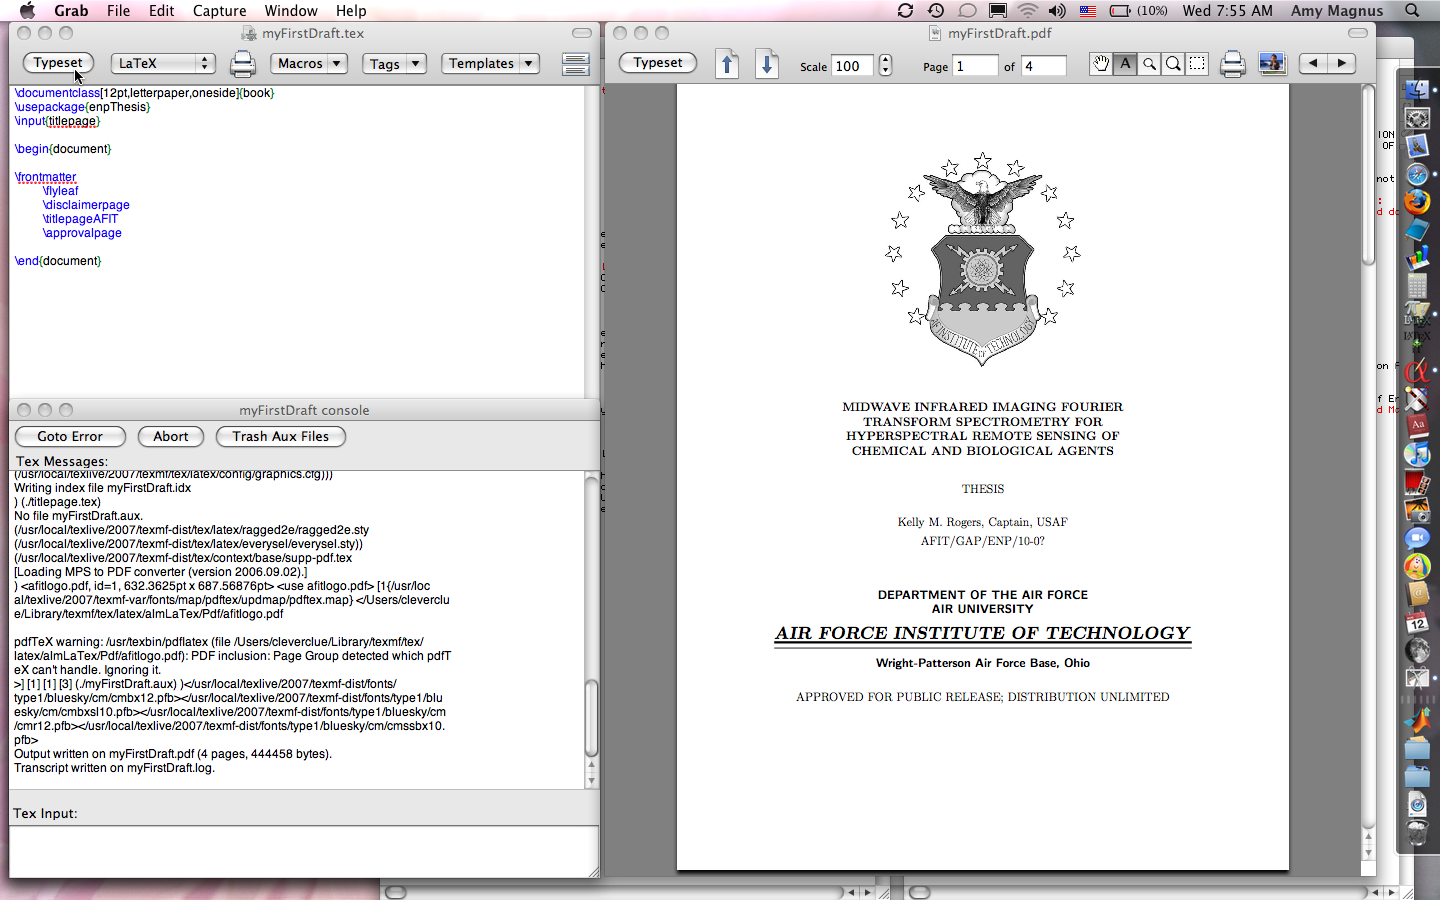
\includegraphics[width=6in]{myFlypage}
     \caption{Here we have compiled the first four page of a thesis.}
     \label{fig:myFlypage}
 \end{center}
\end{figure}
}

\newcommand{\figmyFirstAbstract}{\begin{figure}[tbp]
 \begin{center}
    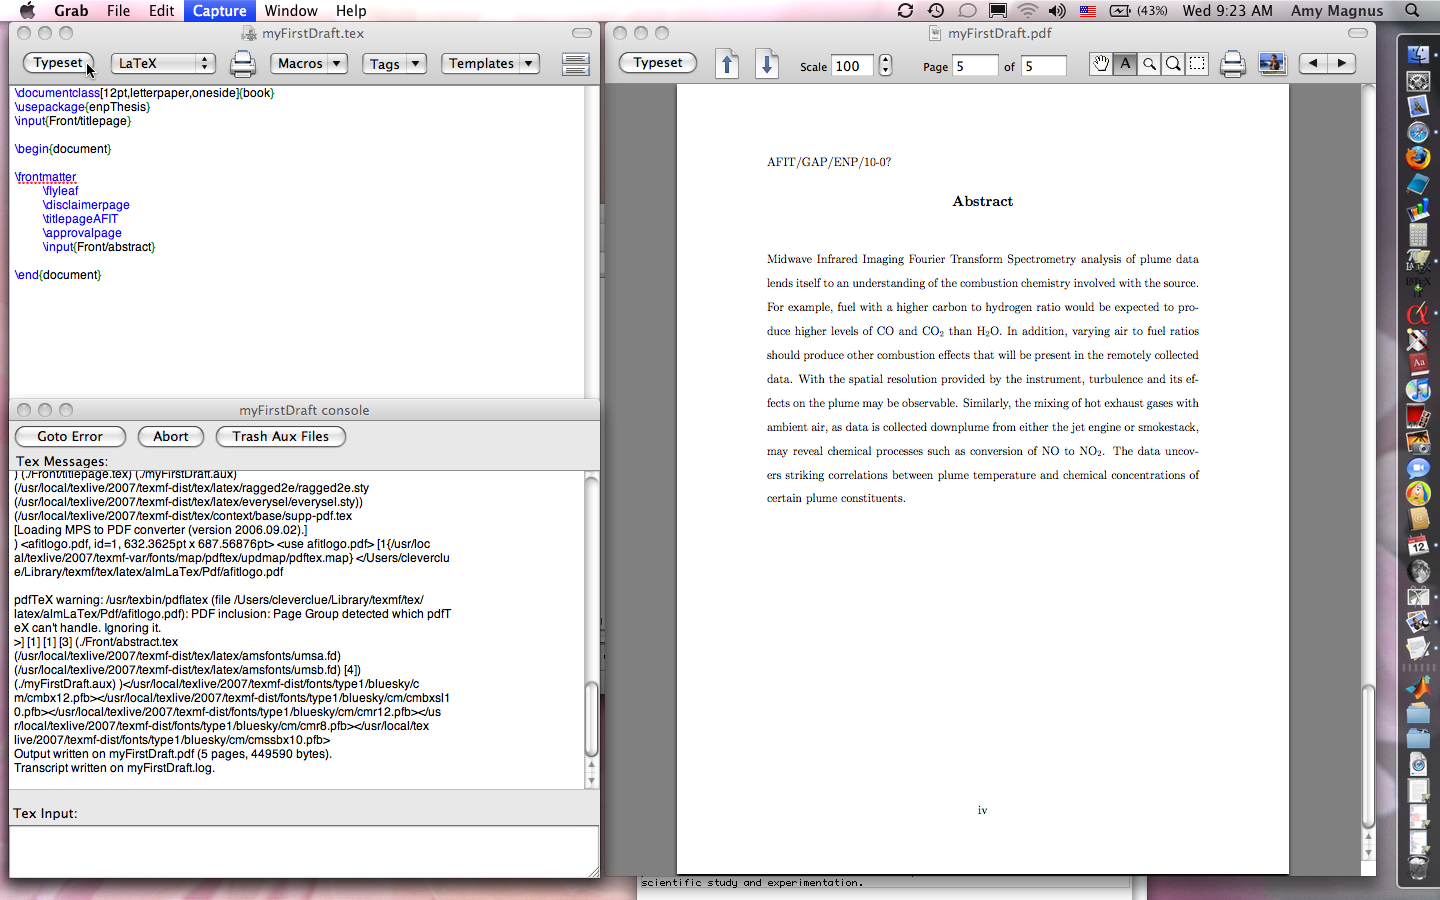
\includegraphics[width=6in]{myFirstAbstract}
     \caption{Add an abstract to the front matter of your thesis.}
     \label{fig:myFirstAbstract}
 \end{center}
\end{figure}
}

\newcommand{\figmyFigures}{\begin{figure}[tbp]
 \begin{center}
    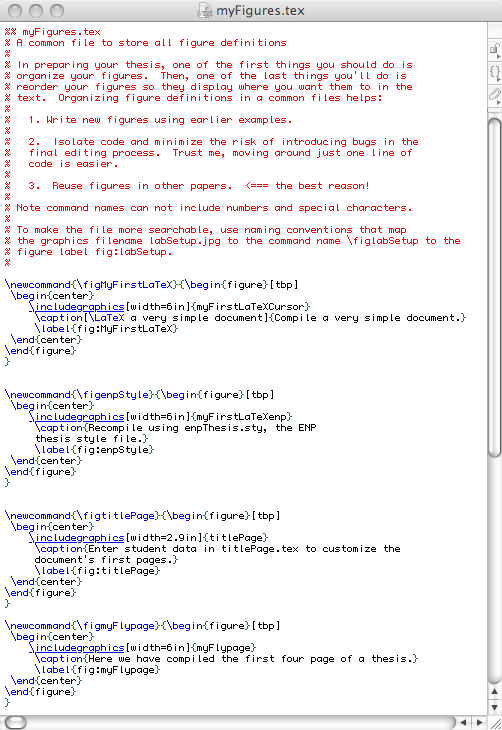
\includegraphics[width=5in]{myFigures}
     \caption{Consider defining all your figures in one file.}
     \label{fig:myFigures}
 \end{center}
\end{figure}
}


\newcommand{\figmyFirstFigures}{\begin{figure}[tbp]
 \begin{center}
    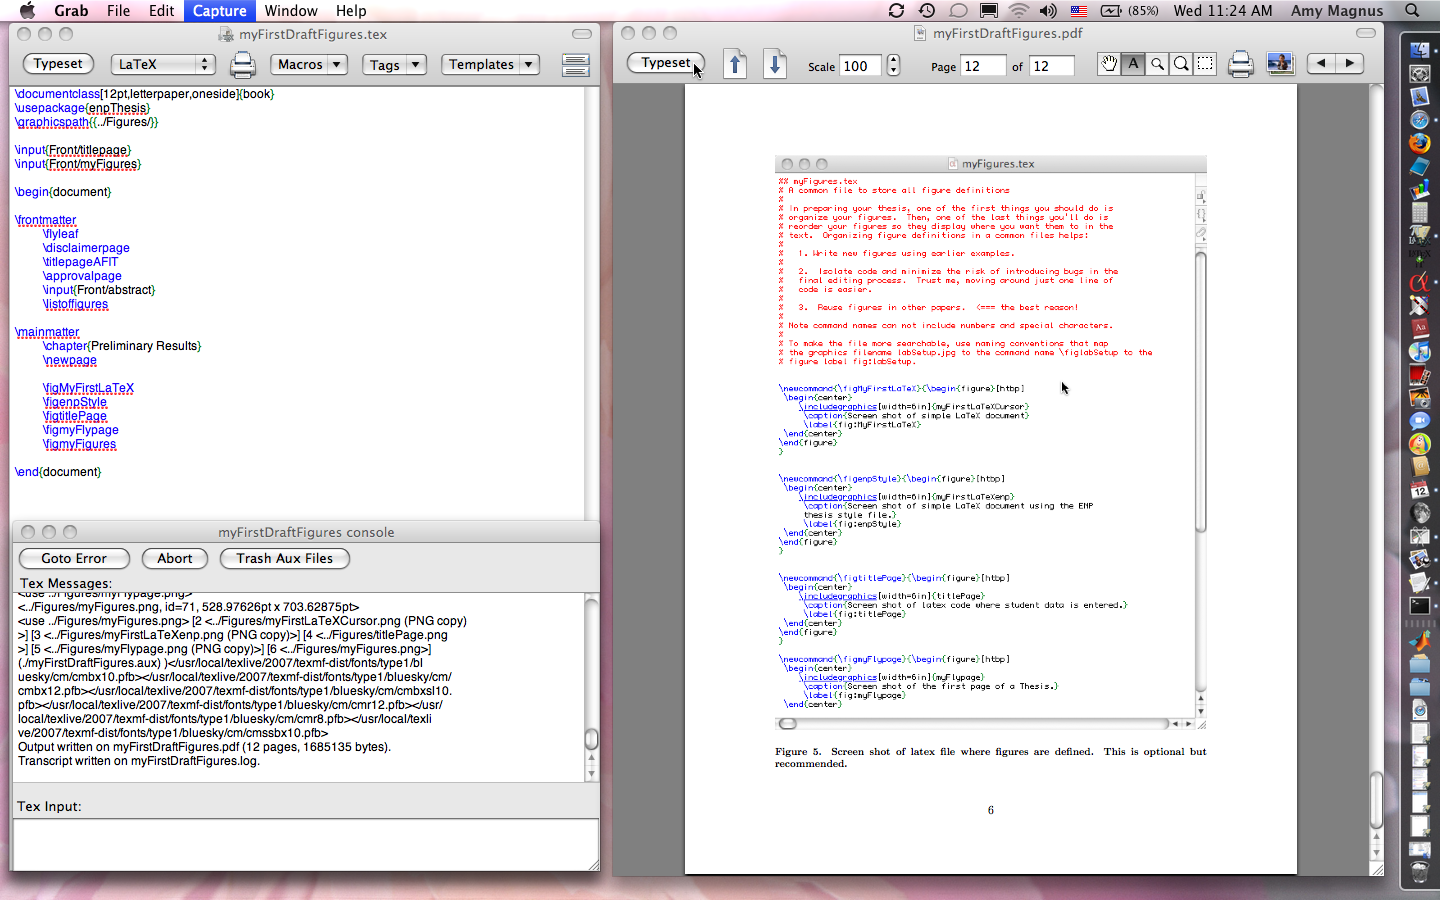
\includegraphics[width=6in]{myFirstFigures}
     \caption{Add figures in the main matter of your document; fill in
     the document around your graphics.}
     \label{fig:myFirstFigures}
 \end{center}
\end{figure}
}

\newcommand{\figmyFirstBibTeX}{\begin{figure}[tbp]
 \begin{center}
    \includegraphics[width=6in]{myFirstBibTeX}
     \caption{Add your bibliography.}
     \label{fig:myFirstBibTeX}
 \end{center}
\end{figure}
}




% define custom commands
\newcommand{\regmark}{\raisebox{5pt}{\tiny \circledR}\xspace}
\newcommand{\matlab}{\textsc{Matlab}\regmark}
\newcommand{\trademark}{\raisebox{5pt}{\tiny TM}\xspace}
\newcommand{\mca}{\texttt{Mathematica}\regmark}
\newcommand{\Latex}{\LaTeX\xspace}

% Create a new theorem style called a Corollary.
% If you don't have any, then just comment this out.
%\theoremstyle{plain} % Default
\newtheorem{cor}{Corollary}[chapter]

%Custom Commands for Student

\newcommand{\primerAddress}{{L:$\backslash$Courses$\backslash$PHYS$\backslash$LaTeX}\xspace}


\begin{document}
\frontmatter
        \flyleaf                        
        \disclaimerpage                 
        \titlepageAFIT                      
        \committeepage  
        % !TEX root = ../SteadmanThesis.tex
\begin{abstract}
Storm enhanced densities (SEDs) are ionospheric plasma enhancements that disrupt radio communications in the near-Earth space environment, degrading the Global Positioning System (GPS) and other high-frequency systems.  Accurate GPS/total electron content (TEC) correction maps produced by ionosphere models can mitigate degradations from SEDs.  An artificial SED was created and ingested via slant TEC measurements into the Global Assimilation of Ionospheric Measurements Gauss-Markov Kalman Filter Model to determine how many ground GPS receivers are needed to produce reliable GPS/TEC correction maps over the continental United States during geomagnetic storming.  It was found that 110 well-positioned GPS receivers produced the best overall TEC accuracy, although significantly improved accuracy was still achieved if 40 or more receivers were used.  It was determined that receiver positioning had a greater impact on TEC accuracy than the number of receivers.  Additionally, it was found that TEC accuracy for the SED region increased at the expense of TEC accuracy everywhere else on the map.
\end{abstract}


        \tableofcontents
        \listoffigures
        

\begin{preface}
Welcome to the world of \Latex! Learn \Latex and you can rapidly
produce papers tailored for a wide variety of publications.
When you create a digital
document\ldots whether you use a ``what you see is what you get''
(WYSIWYG) interface like Microsoft Word or a typesetting system like
\Latex\ldots you are writing a program.  In the realm of academic publishing,
\Latex helps us write a better program.   

The best reasons to write with \Latex are high quality equations,
superior graphics, and the automated generation of table of contents,
lists, and bibliographies.  We can create clean 50+ page documents
that reformat in a snap.  Additionally, due to the fact that the
\Latex typesetting system was written by and for academics, many
of its tools are free and run on Microsoft Windows, Mac OS X, and
Linux.

So let's get started.  Download a \Latex distribution for 
your computer platform, set up your editor and compiler and we'll get 
cracking.  
\end{preface}



\mainmatter
        \chapter{The First Steps}
                Take the first steps in writing your thesis using the simple programs
described in this chapter as a guide.  The source code and support files can be
found on the student drive \primerAddress.  With a
current \Latex distribution\footnote{\Latex distributions update
annually in June.  As of June 2014, the current \Latex
distributions are MiKTeX 2.9 for Windows, TeX Live 2014 for Linux, and
MacTeX 2014 for Macintosh.}, you will be able to compile these programs
without hiccup.

The directory tree below provides a recommended file structure
for the papers generated in your research.  Directories follow ``$>$'' signs; 
standared\ files are
specified in parentheses. 
{\singlespace
\begin{lstlisting}
> myLatexDocuments
  >> afitStyleFiles (afitThesis.sty)
  >> Figures (afitlogo.pdf, afitlogo.eps)
  >> Thesis  (myThesis.tex)
     >>> Preamble (titlePage.tex,myFigures.tex)
     >>> Front (abstract.tex)
     >>> Chapter01 (sectionOne,sectionTwo,...)
     >>> Chapter02 
     . . .
     >>> Appendix01
     . . .
  >> Archived Draft of Thesis 
  >> Archived Perspectus 
  >> Paper One
  >> Paper Two
\end{lstlisting}
} \noindent In a parent directory, create three directories
``afitStyleFiles'', ``Figures'', and ``Thesis''.  Place your graphics
(such as afitlogo.pdf) in the directory Figures, your \Latex style
files (afitThesis.sty, sf298.sty, sf298.dtx, and sf298.ins) in
afitStyleFiles, and the latex code for your thesis document in Thesis.
Organized in this way, the files in the Figures directory and the
afitStyleFiles directory can be used by your thesis, perspectus, archived drafts,
and other publications.  Typically, graphics account for most of the
memory taken up by a digital document, and this efficiency in
sharing saves significant disk space.



		
                \figMyFirstLaTeX
                \section{\Latex a simple document}
                To compile a LaTex document, start simple with the code listed 
below.  Store the code as a .tex file in your
Thesis directory. Then compile the code to test the set up of your \Latex 
distribution and compiler\footnote{Popular compilers include TeXworks 
and TeXShop.}.  Figure~\ref{fig:MyFirstLaTeX} provides a screen
shot of the typeset document with its compilation aids.

 {\singlespace   
 \begin{verbatim}
\documentclass[12pt,letterpaper,oneside]{book}
 
\begin{document}
The quick brown fox jumped over the lazy dog.
\end{document}
\end{verbatim}
} 
\noindent The code has two parts: the preamble and the body.  The
preamble establishes the default formatting for the document; the body
holds the content.  The preamble starts with a {\bf $\backslash$documentclass}
declaration and ends at the {\bf $\backslash$begin\{document\}}
command. The {body} is placed in between the {\bf
$\backslash$begin\{document\}} and {\bf $\backslash$end\{document\}}
commands. 

In the preamble of this first document, Here we have selected a one
sided, 12-pt font book format.  In the body, let us enter a short
phrase---just to get a feel for how content is added---that includes 
all characters in the Roman alphabet.
    
   
%Other formats include article, report, memoir The body contains the
%actual content.


		

                \figafitStyle
                \section{Add a style file}
                Next, we add the style file afitThesis.sty to the preamble and
recompile.  The style file implements the AFIT thesis format and is
added via the command {\bf $\backslash$usepackage}.

\vspace{-0.3in}
{\singlespace
\begin{verbatim}
\documentclass[12pt,letterpaper,oneside]{book}
\usepackage{../afitStyleFiles/afitThesis}

\begin{document}
The quick brown fox jumped over the lazy dog.
\end{document}
\end{verbatim}
} \noindent Note the resulting changes to the document in
Figure~\ref{fig:afitStyle}.  Some adjustments are immediately apparent:
The margins have changed and a page number is now located at the
bottom of the page.
    

		

                \figtitlePage
                \section{Add the front matter}
                The style file {\em afitThesis.sty} contains code that generates the
first, standardized pages of the thesis document.  Theses pages are the
flyleaf, disclaimer page, the title page, and the committee page.  For
each thesis, we customize these four pages by editing a tex file
called {\em titlePage.tex}.  The customizable items for a thesis are:

\vspace{-0.15in}
\begin{tabular}{p{2.2in}p{4in}}
    \begin{itemize}\itemsep-10pt
	    \item Author
	    \item Rank
	    \item Graduation Date
	    \item Document Designator
	    \item Flypage title
	    \item Title
     \end{itemize} &
    \begin{itemize}\itemsep-10pt
	    \item Previous degrees
	    \item Academic degree upon AFIT graduation
	    \item Committee membership
	    \item Department granting your degree
	    \item School address
	    \item Distribution statement
	    \item Disclaimer
     \end{itemize} 
\end{tabular}

\noindent Add this information to {\em titlePage.tex} as you obtain
it.  One item to include as soon as possible is the distribution
statement; ask your advisor which distribution statement is
appropriate for your draft document.
    
If your document is something other than a thesis, you can set a flag at
the beginning of {\em titlePage.tex}.  Use the $\%$ symbol to comment
out unused flags and remove the $\%$ from the line of the
appropriate flag.  In this way, the correct flag will execute at
compilation.  The available flags correspond to the following
documents:

\vspace{-0.3in}
{\singlespace
\begin{center}
\begin{tabular}{|l|l|}
    \hline
    \bf Document & \bf Flag\\
    \hline
    Thesis & {\bf $\backslash$afitthesis}  \\
    Report & {\bf $\backslash$afitreport} \\
    Dissertation & {\bf $\backslash$dissertation} \\
    Prospectus & {\bf $\backslash$prospectus}\\
    \hline
\end{tabular}
\end{center}}

Once you customize the {\em titlePage.tex} file, we can typeset
the first four pages of an AFIT thesis: the flypage, the disclaimer
page, the title page and the committee page. 

We must add a few lines to our typesetting program.  Within the
document environment, we list the first four pages (See line 7-11)
under front matter.  The flypage includes our first graphic---the AFIT
logo---so we provide a path to our figures by using the {\bf
$\backslash$graphicspath} command\footnote{Note the double brackets
used in the graphicspath command; they are necessary for the command
to execute properly with some compilers.} in the preamble.  Note line
3 below where we set the path.  The {\em titlePage.tex} provides
customization, not content, so it is called in the preamble;
call the file by using the command {\bf $\backslash$input} as in line
4 of the code below.  In all, we have added seven lines of code to our
short program to create a four page document.

\vspace{-0.25in}
{\singlespace
\begin{verbatim}
\documentclass[12pt,letterpaper,oneside]{book}
\usepackage{afitThesis}
\graphicspath{{..\Figures}}
\input{Preamble/titlepage}

\begin{document}
\frontmatter
        \flyleaf                        
        \disclaimerpage                 
        \titlepageAFIT                      
        \committeepage  	
\end{document}
\end{verbatim}
}


                \figmyFlypage
                
\noindent The next section to add to the front matter is an abstract.
Create a file {\em abstract.tex} and place the text for the abstract
between the commands {\bf $\backslash$begin\{abstract\}} and {\bf
$\backslash$end\{abstract\}} as below.

\vspace{-0.3in}
{\singlespace
\begin{verbatim}
\begin{abstract}
    Midwave Infrared Imaging Fourier Transform Spectrometry analysis of
    plume data lends itself to an understanding of the combustion
    chemistry involved with the source. ...
\end{abstract}
\end{verbatim}
}

Above, we use a construct called an environment.  There are several
enviroments: figure, itemize,
verbatim, quote, equation to name a few.  \Latex friendly editors will
help you build these environments.  The abstract environment is
actually a customized environment created in the {\em afitThesis.sty}
file; thus, it will not be found in the common \Latex literature or
tools; but, as you can see above, it is simple to implement.



                \figmyFirstAbstract
                Other common items that can be added to the front matter are
acknowledgements, the table of contents and lists of figures and
tables.  The acknowledgements can be added in the same manner as the
abstract; use the environment commands for the
Acknowledgement: {\bf $\backslash$begin\{acknowledgement\}} and {\bf
$\backslash$end\{acknowledgement\}}.  The table of contents and other lists
build automatically as you add sections, figures, and tables and are placed
in the front matter using the commands below.  

\vspace{-0.3in} {\singlespace
\begin{verbatim}
\frontmatter
        \flyleaf                        
        \disclaimerpage                 
        \titlepageAFIT                      
        \committeepage
        \input{Front/abstract}
        \input{Front/acknowledgement}
        \tableofcontents
        \listoffigures
        \listoftables
\end{verbatim}
}

\noindent The order follows the AFIT style guide\cite{AFITStyle}.  The {\em
afitThesis.sty} defines additional environments and lists.  We
will describe how to implement those items in the next chapter.
For now, we will simply keep the abstract and perhaps the list of
figures in our front matter as we move on to the
main body of the thesis.






                \section{Add figures to the main matter and start writing}
                \figmyFigures
                
To concentrate on your research, consider organizing your figures
first.  Build the document around your figures, and you will be able
to concentrate on the story of your contribution---not the work that
has gone on before.  

To organizing your figures, it is helpful to define them in a
common file.  See {\em myFigures.tex} depicted in
Figure~\ref{fig:myFigures} and stored in the Preamble subdirectory.
In this way, you may:
    \begin{itemize}
      \item Readily write new figures using earlier examples. 
      
      \item  Isolate code and minimize the risk of introducing bugs in the
      final editing process.  Moving around one line of
      code is easy and safe.
      
      \item Standardize figures without having to locate them 
      throughout the document.
      
      \item  Reuse figures in other papers.  $\leftarrow$ The best reason!
    \end{itemize}
        
\noindent In {\em myFigures.tex}, use {\bf
$\backslash${newcommand}} to define a command for each figure as
below:

{\vspace{-.30in}}
{\singlespace
\begin{verbatim}
\newcommand{\figmyFigures}{
    \begin{figure}[htbp]
        \begin{center}
             \includegraphics[width=6in]{myFigures}
             \caption{A sample tex file where figures are defined.}
             \label{fig:myFigures}
        \end{center}
    \end{figure}
}
\end{verbatim}}
    
\noindent For a command, chose a naming convention that
intuitively links the command to the graphic file and the figure
label.  For example, above we have defined a command {\bf
$\backslash${figmyFigures}} to position a figure containing graphic
myFigures.png.  Note command names cannot include numbers or special
characters.



                \figmyFirstFigures
                
Now, in the preamble of your code, input {\em myFigures.tex} in the
same manner as you input {\em titlepage.tex}.  Now we are ready to add
the main body of the thesis.  Initiate the main body of your document
by calling the {\bf$\backslash$mainmatter} command.  Next, call the
figures that you have defined and compile.  Note, once you add a
chapter, you can remove {\bf$\backslash$thispagestyle\{plain\}} which
precedes the {\bf$\backslash$mainmatter} command.

\vspace{-0.3in}
{\singlespace
\begin{verbatim}
\documentclass[12pt,letterpaper,oneside]{book}
\usepackage{afitThesis}
\graphicspath{{..\Figures}}
\input{Preamble/titlepage}
\input{Preamble/myFigures}

\begin{document}
\frontmatter
        \flyleaf                        
        \disclaimerpage                 
        \titlepageAFIT                      
        \committeepage  	
        \input{Front/abstract}
        \tableofcontents
        \listoffigures
\mainmatter
        \figMyFirstLaTeX
        \figafitStyle
        \figtitlePage
        \figmyFlypage
        \figmyFirstAbstract
        \figmyFigures
        \figmyFirstFigures
\end{document}
\end{verbatim}
}
\vspace{-0.1in}

From here, add text around your figures.  To produce this document, we
used the following code:

\vspace{-0.25in}
{\singlespace
\begin{verbatim}
\documentclass[12pt,letterpaper,oneside]{book}
\usepackage{afitThesis}
\graphicspath{{../Figures/}}

\input{Preamble/titlepage}
\input{Preamble/myFigures}
\input{Preamble/commonSymbols}

\begin{document}
\frontmatter
        \flyleaf                        
        \disclaimerpage                 
        \titlepageAFIT                      
        \committeepage  
        \input{Front/abstract}
        \tableofcontents
        \listoffigures
        \input{Front/preface}
\mainmatter
        \chapter{The First Steps}
                \input{chapter01/mySetup}		
                \figMyFirstLaTeX
                \section{\Latex a simple document}
                \input{chapter01/startSimple}		

                \figafitStyle
                \section{Add a style file}
                \input{chapter01/addStyle}		

                \figtitlePage
                \section{Add the front matter}
                \input{chapter01/addFrontMatter}
                \figmyFlypage
                \input{chapter01/addAbstract}
                \figmyFirstAbstract
                \input{chapter01/addMoreFrontMatter}

                \section{Add figures to the main matter and start writing}
                \figmyFigures
                \input{chapter01/addFirstResults}
                \figmyFirstFigures
                \input{chapter01/addMainMatter}
\end{document}
\end{verbatim}
}
\vspace{-0.25in}


\end{document}
\end{verbatim}
}
\vspace{-0.25in}


\end{document}
\end{verbatim}
}
\vspace{-0.25in}


\end{document}
\end{verbatim}
}
\vspace{-0.25in}

